\documentclass[UTF8]{ctexart}
\usepackage{hyperref}
\usepackage{graphicx}
\usepackage{subfigure}
\usepackage{float}
\usepackage{caption}
\usepackage{longtable}
\pagestyle{plain}
\hypersetup{
  colorlinks=true,
  linkcolor=blue,
  filecolor=blue,
  urlcolor=blue,
  citecolor=cyan
}
\captionsetup[figure]{font=normalsize}
\begin{document}
\title{关于Big5人格测验的探索性分析报告}
\author{刘哲}
\maketitle
\part{背景介绍}
\section{人格测验}
世界上没有两片相同的树叶,同样,世界上也没有完全相同的两个人。
与树叶不同,人与人之间的差异不光体现在外表上,还更多的体现在人格上。
俗话说,“画虎画皮难画骨,知人知面不知心”,一个人的外表如何,我们很容易就能形容出来;
但是一个人的人格如何,单薄的语言很难完整准确地描述,而且人格评价的主观性极强,
“一千个人有一千个哈姆雷特”,没有统一的评价标准。
为了满足人们深入了解自身或他人人格特点的需要,
诞生了用于测试并解释个人行为独特性和倾向性等特征的测验形式,
称为人格测验($personality\ test$)。\par
% 人格测验一般采用问卷的方法进行,通过设置一定的场景,引导测验人回答一系列精心设计的问题——
% 一般为没有褒贬的中性问题,将个人的思维方式和行为方式具象化地映射出来,
% 随后可以将个人的各种特征量化成一系列多维度的评分,据此划分出不同的人格类型,
% 或直接以每个人的评分作为人格倾向的测验结果。
人格测验一开始被用于心理学研究,参加者需要填写一份精心设计的测试问卷,
根据每道题目的回答,推断出测试者的人格特质。
人格测验为参与回答同一份测试问卷的人提供了一套统一的人格评价标准,
而且将“人格”这一抽象的概念具体化,比如把人格划分出不同类型或拆分成几个维度指标,
使人格可以在同一个框架内相互比较。\par
% 尽管一次人格测验的结果受到测验人当时心理状态的影响比较大,
% 但也可以通过精心设计问卷题目,或者取多次测验的平均结果,得到一个比较稳健的人格评价。
% 因其有着评价客观、解释容易、可操作性强的优点,人格测验也广泛应用于公司招聘中。
得益于网络的普及,任何人都可以便捷地获得一份人格测验问卷,花上十几分钟填写,
就能得到一份关于自己的人格报告,这种大范围的普及也让人格测验的衍生种类变得越发丰富,
但是按照心理学上对于人格的假说不同,大体都可归为“类型说”和“特质说”两类。
前者认为人格可划分成特定的几种类型,相同人格类型的人会有相似的行为模式,
其中的典型代表是“MBTI十六型人格($Myers-Briggs\ Type\ Indicator$)”;
后者则认为人的行为模式是由一种心理结构引导的,即使是具有不同心理结构的人,
在受到刺激后,也可能表现出类似的行为模式,人格的差异本质上是这种心理结构的差异,
其中的典型代表则是“Big5人格理论($Big\ Five\ Personality\ Traits$)”。
\section{Big5人格理论}
Big5人格理论是人格心理学中“特质流派”的典型代表,发端于人格词汇学研究。
该理论的将词典中描述性格人格特质的词语进行汇总、归类、概括,
将人类创造的所有用于形容人格特质的词汇归为5个维度,
即用开放性($Openness$)、尽责性($Conscientiousness$)、外倾性($Extraversion$)、
宜人性($Agreeableness$)、情绪性($Neuroticism$)5个关键词概括一个人的人格特质。\par
Big5人格理论有其独特的科学性。
首先,由于5个维度源自于词典,我们用来形容人的词基本上不会跳出这个范围,
因此它所得到的结论更容易被人接受和理解。
其次,多个独立的研究都发现人格特质中存在5个最主要的因素,证明“五因素”并非编造。
再次,Big5人格理论属于“特质流派”,它没有将人格分成几种特定的类型,而是采用倾向性分数的形式,
给出测试者更有可能倾向于维度的哪一端,这一点与统计学的思想不谋而合。
最后,5个维度可能是在描述人格时所能达到的最低维度,
著名的“卡特尔十六型人格测验($16PF$)”的作者卡特尔教授也认为,
其16个维度继续降维就是5个维度,而且与“五因素”的维度非常相似。
\section{Big5人格测验}
常用的Big5人格测验有$10-item\ scale$和$20-item\ scale$两个版本
(\href{https://ipip.ori.org/newBigFive5broadKey.htm}{$Big-Five\ Factor\ Markers$}),
分别对应每个维度下10个题目和20个题目,测试者的回答采用“5点量表”,部分题目反向记分。
按维度汇总分数,就得到测试者在5个维度上的人格倾向。
Big5人格测验的5个维度分别是:
\begin{itemize}
  \item $Openness$,开放性:指个体对经验持开放、探求的态度。
        得分高者不墨守成规,更倾向于独立思考;得分低者比较本分,更喜欢实干。
  \item $Conscientiousness$,尽责性:指个体在目标导向行为上的组织、坚持和动机。
        得分高者做事有条理,并能持之以恒;得分低者马虎大意,容易见异思迁,不可靠。
  \item $Extraversion$,外倾性:指个体对外部世界的积极投入程度。
        得分高者热爱交际,精力充沛、乐观、友好;得分低者更加谨慎、冷静,喜欢独处,少说多做。
  \item $Agreeableness$,宜人性:指个体在合作与社会和谐性方面的差异。
        得分高者富有同情心,更注重合作;得分低者喜欢为了自己的利益和信念而奋斗。
  \item $Neuroticism$,情绪性:指个体体验消极情绪的倾向。
        得分高者更容易烦恼和焦躁,出现情绪化反应;得分低者擅长自我调节,不易出现极端反应。
\end{itemize}
将维度名称的首字母连起来,Big5人格模型也被称为OCEAN模型。\par
必须强调,五个维度上的得分高低只能代表特质的倾向,不代表人格的优劣。
\part{数据来源和预处理}
\setcounter{section}{0}
\section{研究目的与数据来源}
前面提到,Big5人格测验的结果是5个维度上代表特质倾向的分数,
虽然它很好地将“人格”这一概念量化了,但没有给出明确的高低分界限,也不便于形成浅显易懂的文字描述。
一个维度上高于多少分才算高分,低于多少分才算低分?
如何通过5个维度上的分数区分出人们的人格特质差异?都有很大的解释空间。\par
本文使用的数据为人格测验网站\href{https://openpsychometrics.org}{$Open\ Psychometrics$}
收集的测验数据,测验问卷为$10-item\ scale$版,且测试者均同意其测验结果用于科学研究。
原始数据包含$1,015,341$条测验数据,变量名以“维度+题号”的格式对应50道题目,
以英文缩写OPN、CSN、EXT、AGR、EST依次表示五个维度,以数字1$\sim$10表示题号,
数据值为表示是否同意题目描述的“五点量表”,
“1”表示“完全同意”,“2”表示“同意”,“3”表示“中立”,“4”表示“不同意”,“5”表示“完全不同意”。\par
% 除此之外,数据中还有一些参加测验者的个人信息,考虑到数据的准确性和可用性,
% 仅保留参加者的国家信息,用于研究国家之间人格特质的差异。
由于样本量足够大,且测试者分布范围很广,认为利用该数据得到的结论具有一般性。
\section{数据清洗和数据预处理}
\subsection*{删除无效数据}
首先,原始数据中存在可能是由数据采集失误造成的无效数据,共有$1,783$条。\par
此外,由于测试者没有被要求必须回答全部题目,数据中存在部分记录为“0”的缺失值。
缺失值数据被分成两部分处理:第一,鉴于每个维度下仅有10道题目,
认为全部题目中缺失回答数大于等于6个属于严重缺失,这部分数据同样被视作无效数据,共有$5,368$条;
第二,认为缺失回答数小于等于5个属于不严重缺失,共有$133,756$条。\par
删除$7,151$条无效数据后得到$1,008,190$条有效数据,其中的$133,756$条数据含有缺失值,
约占$13\%$,删去这部分数据会损失较多信息,需要对其进行补数。
\subsection*{填补缺失值}
Big5人格测验被设计成用10道题目来推断测试者在该维度上的人格特质,那么反过来,
同一维度上具有相同人格特质的人在这10个题目会有相同的回答,因此选择$K$最近邻方法填补缺失值。\par
具体做法为:计算含缺失值数据与完整数据之间的欧氏距离;
选择与含缺失值数据最相近的10条完整数据,根据距离越近、权重越高的原则确定权重;
计算10条数据的加权平均,填补对应的缺失值。\par
过程中有两点需要注意:一是每个变量的取值范围均为1$\sim$5,而且不同的取值都有各自的实际意义,
补数需要找到缺失值有可能的真值,因此计算距离时可以不将数据标准化;
二是加权平均的结果会包含小数部分,要将其四舍五入为整数作为最终补数。
\subsection*{数据预处理}
数据清洗后得到$1,008,190$个样品,后续的分析中对数据有一些预处理。\par
在计算一个维度的总分时,正向记分的题目可以直接将表示符合程度的1$\sim$5作为该题目的分数,
但部分反向记分的题目对应分数为5$\sim$1。\par
在聚类分析时,使用公式
\begin{equation}
  DimScore\_scale = \frac{DimScore\_origin - 30}{20}
  \label{scale}
\end{equation}
将维度总分的的取值范围由10$\sim$50变为-1$\sim$1,总分小于零代表低分倾向,总分大于零代表高分倾向,
% 这样“完全不同意”对应到“-1”,“中立”对应到“0”,“完全同意”对应到“1”,然后计算维度总分,
更方便理解和比较,需要时可以通过逆变换变回原取值范围。
\part{数据可视化分析}
\setcounter{section}{0}
\section{题目分数的分布}
理论上,每道题目分数的分布图像应该近似于对称的钟形,
即大多数人会选择“中立”,较少人会选择“完全不同意”或“完全同意”。
实际中,人们的选择与问题描述有很强的关联。
题目越接近普适的道德标准、越是抽象笼统的描述,测试者越倾向于认同态度,
此时分布图像会更陡峭,且呈现偏态或单调的形态;
反之,越接近崇高的个人品质、越是精确的具体描述,测试者越倾向于中立态度,
此时分布图像会更平缓,且接近对称的形态。\par
统计每个题目下各个分数的人数,画出条形图如下:
\begin{figure}[H]
  \centering
  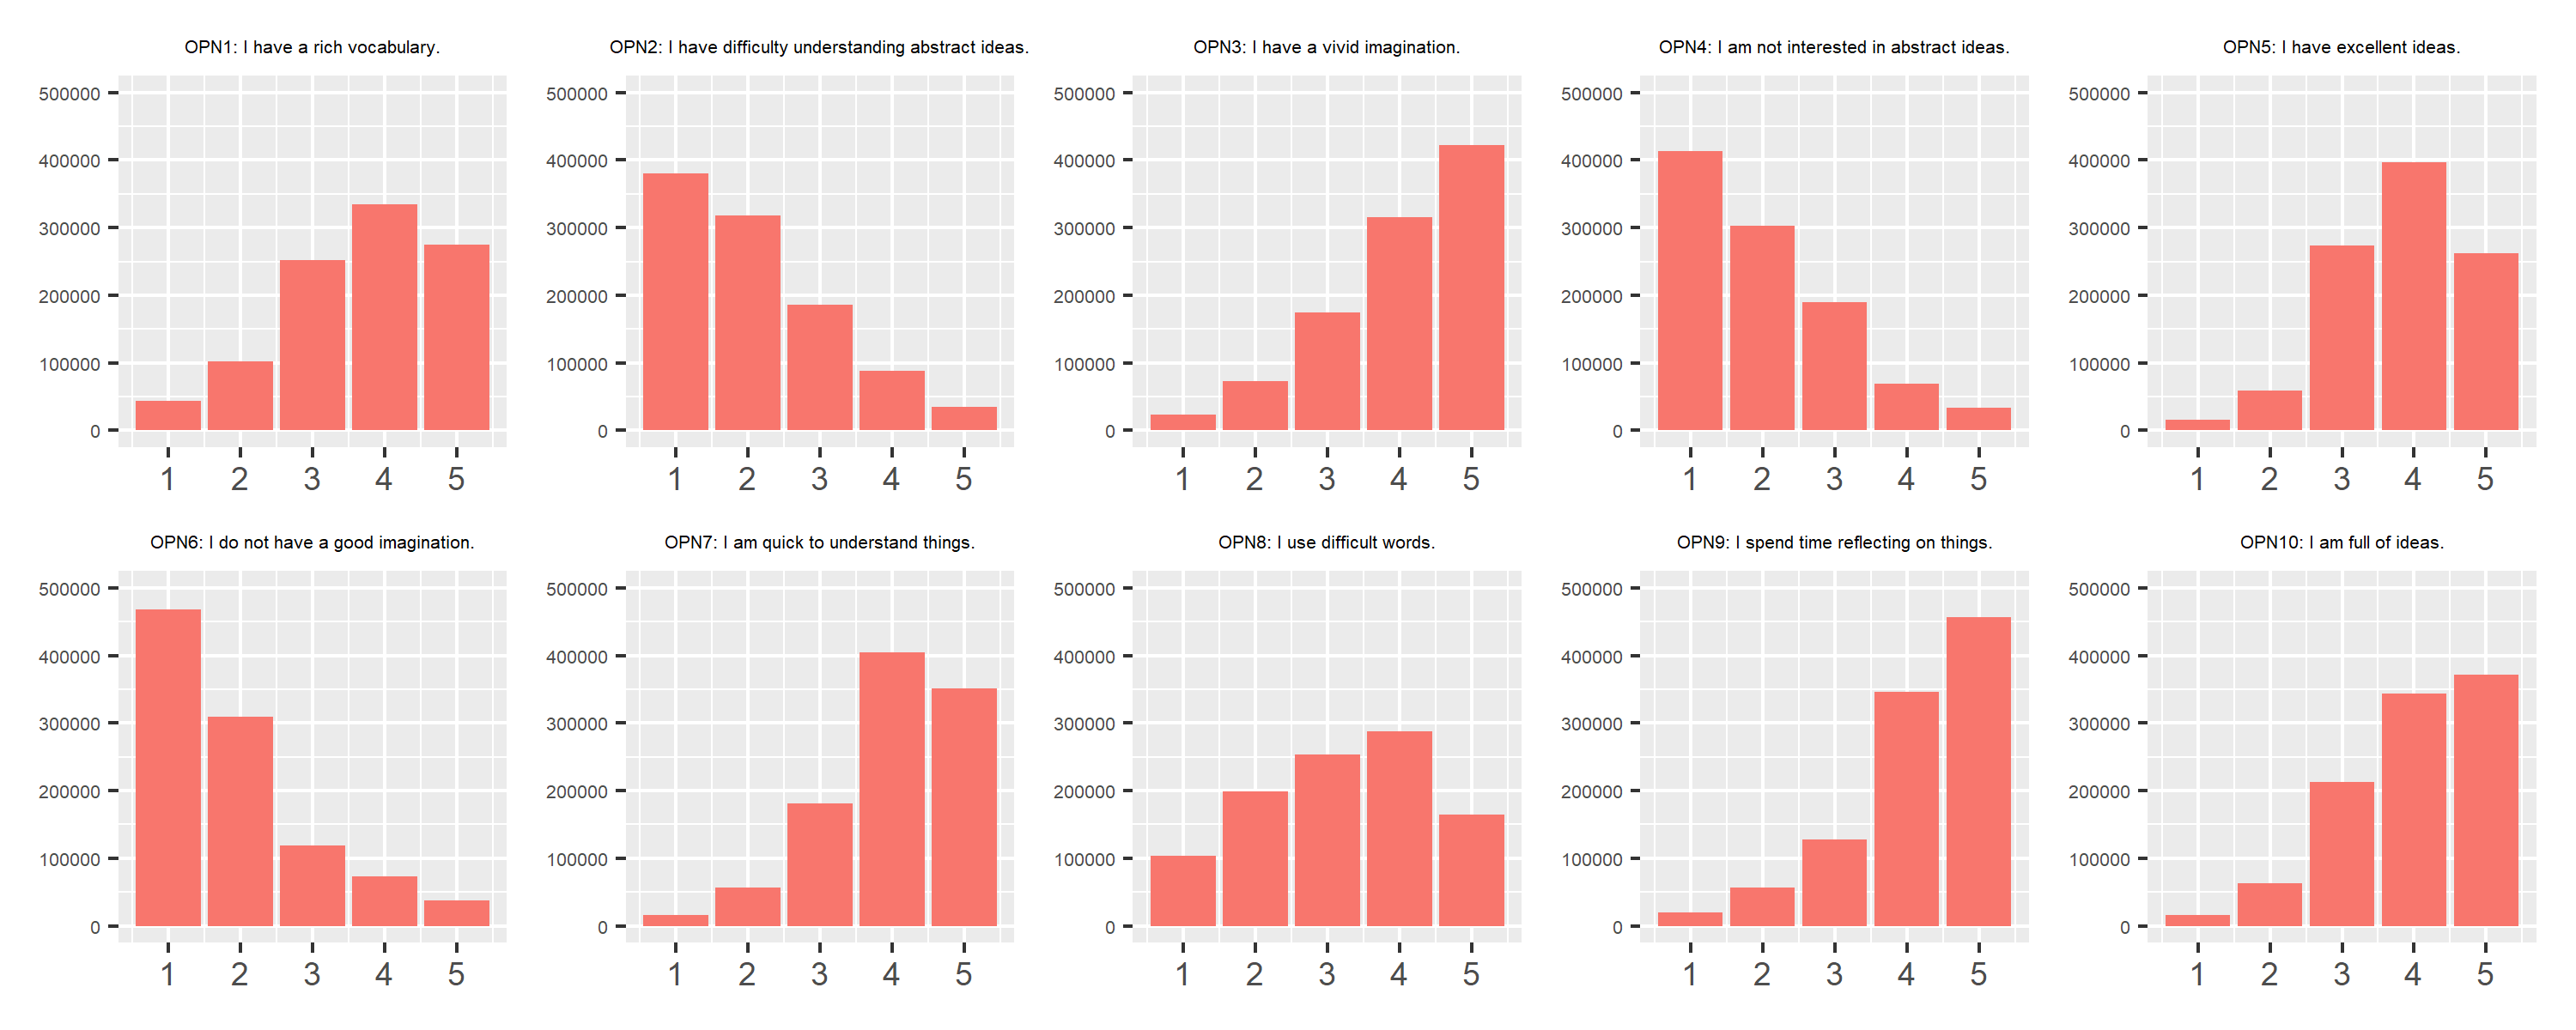
\includegraphics[scale=0.478]{OPN.png}
  \caption{开放性维度的题目及人数分布}
\end{figure}
\begin{figure}[H]
  \centering
  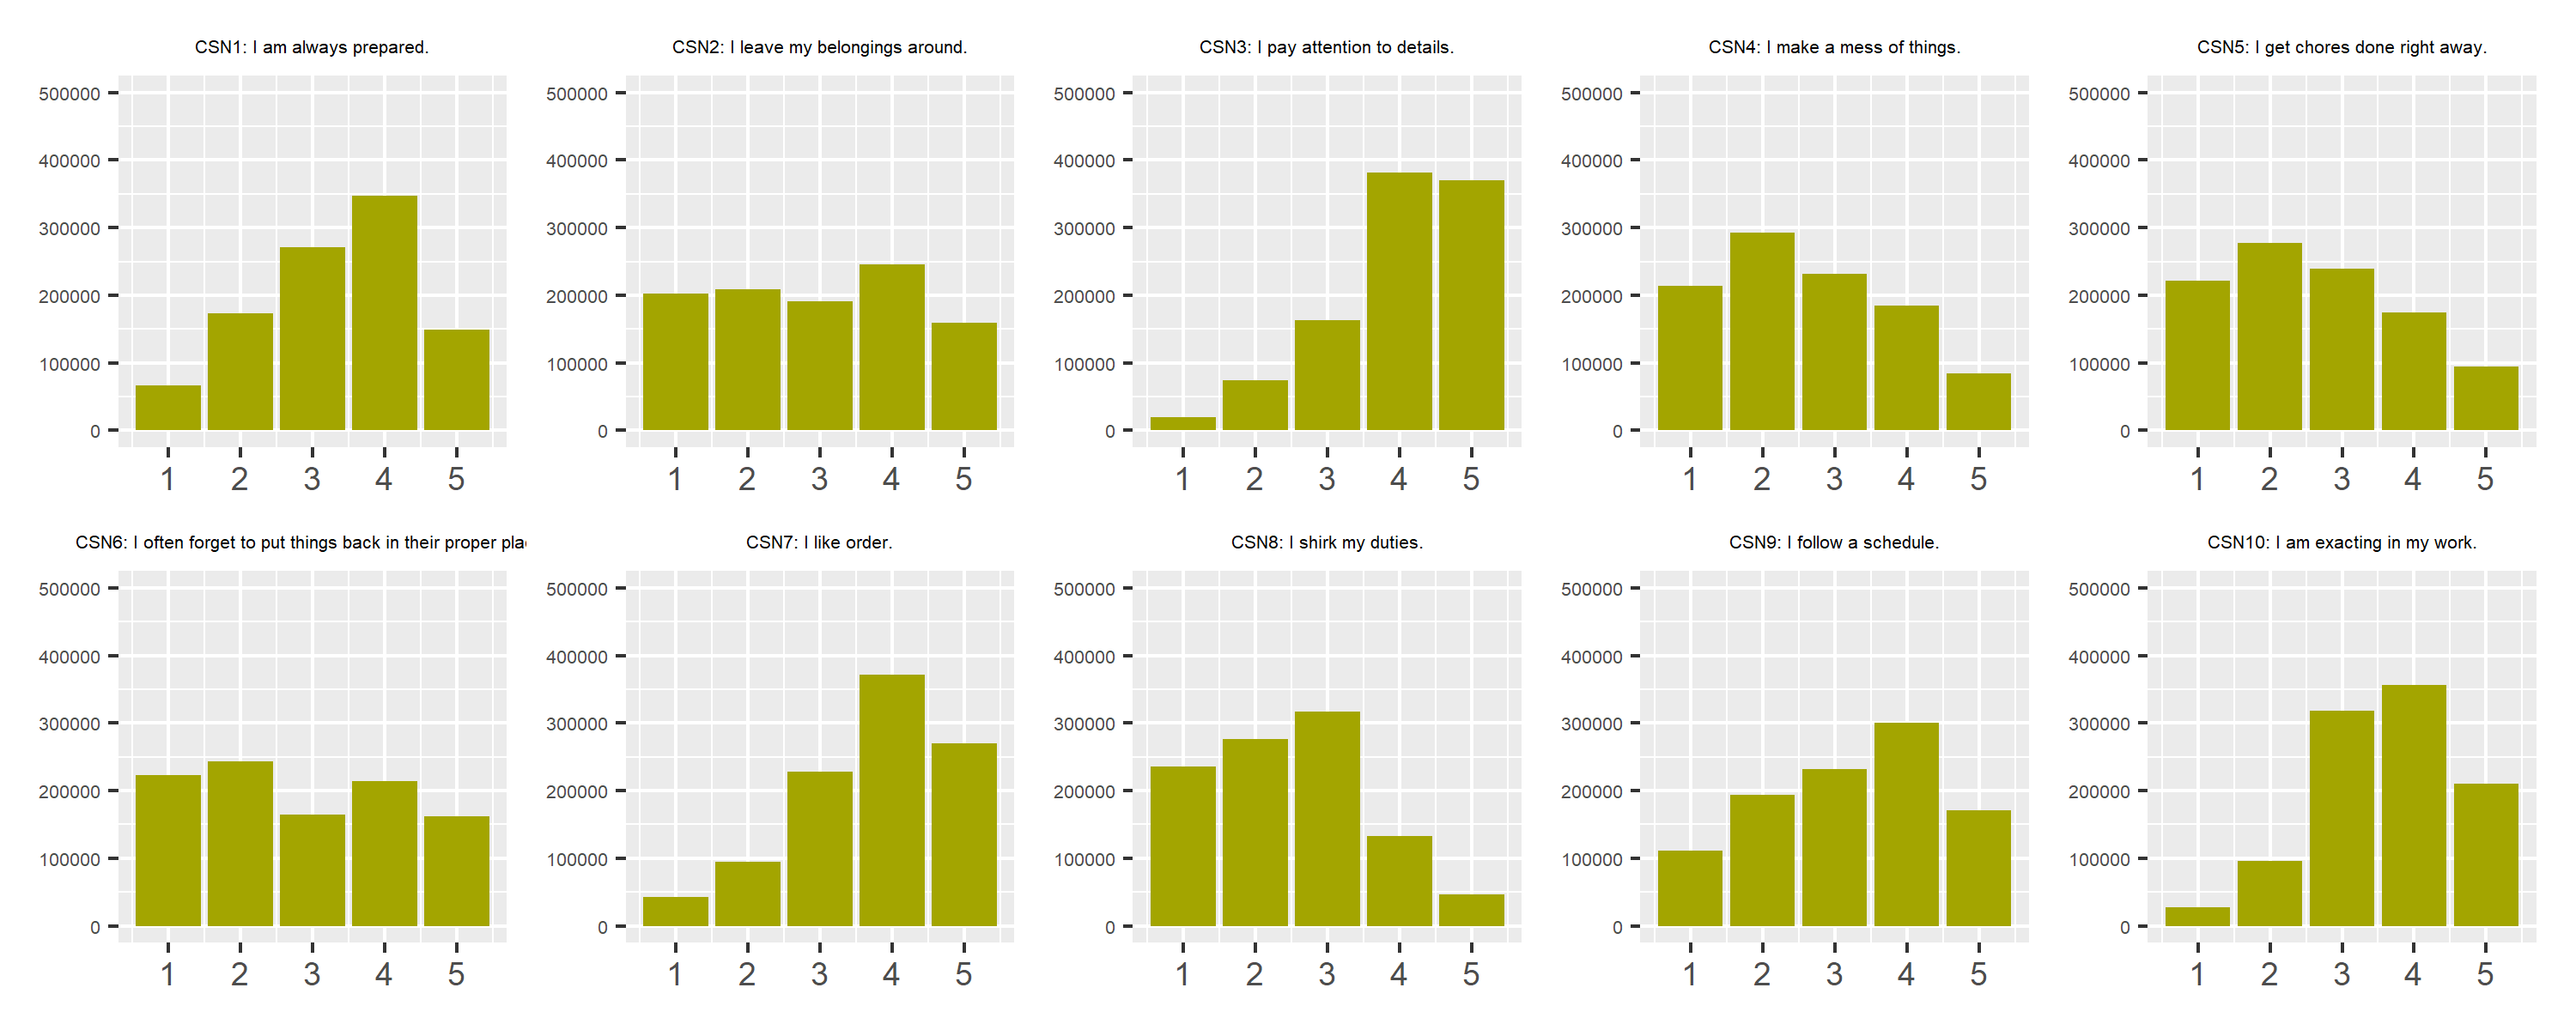
\includegraphics[scale=0.478]{CSN.png}
  \caption{尽责性维度的题目及人数分布}
\end{figure}
\begin{figure}[H]
  \centering
  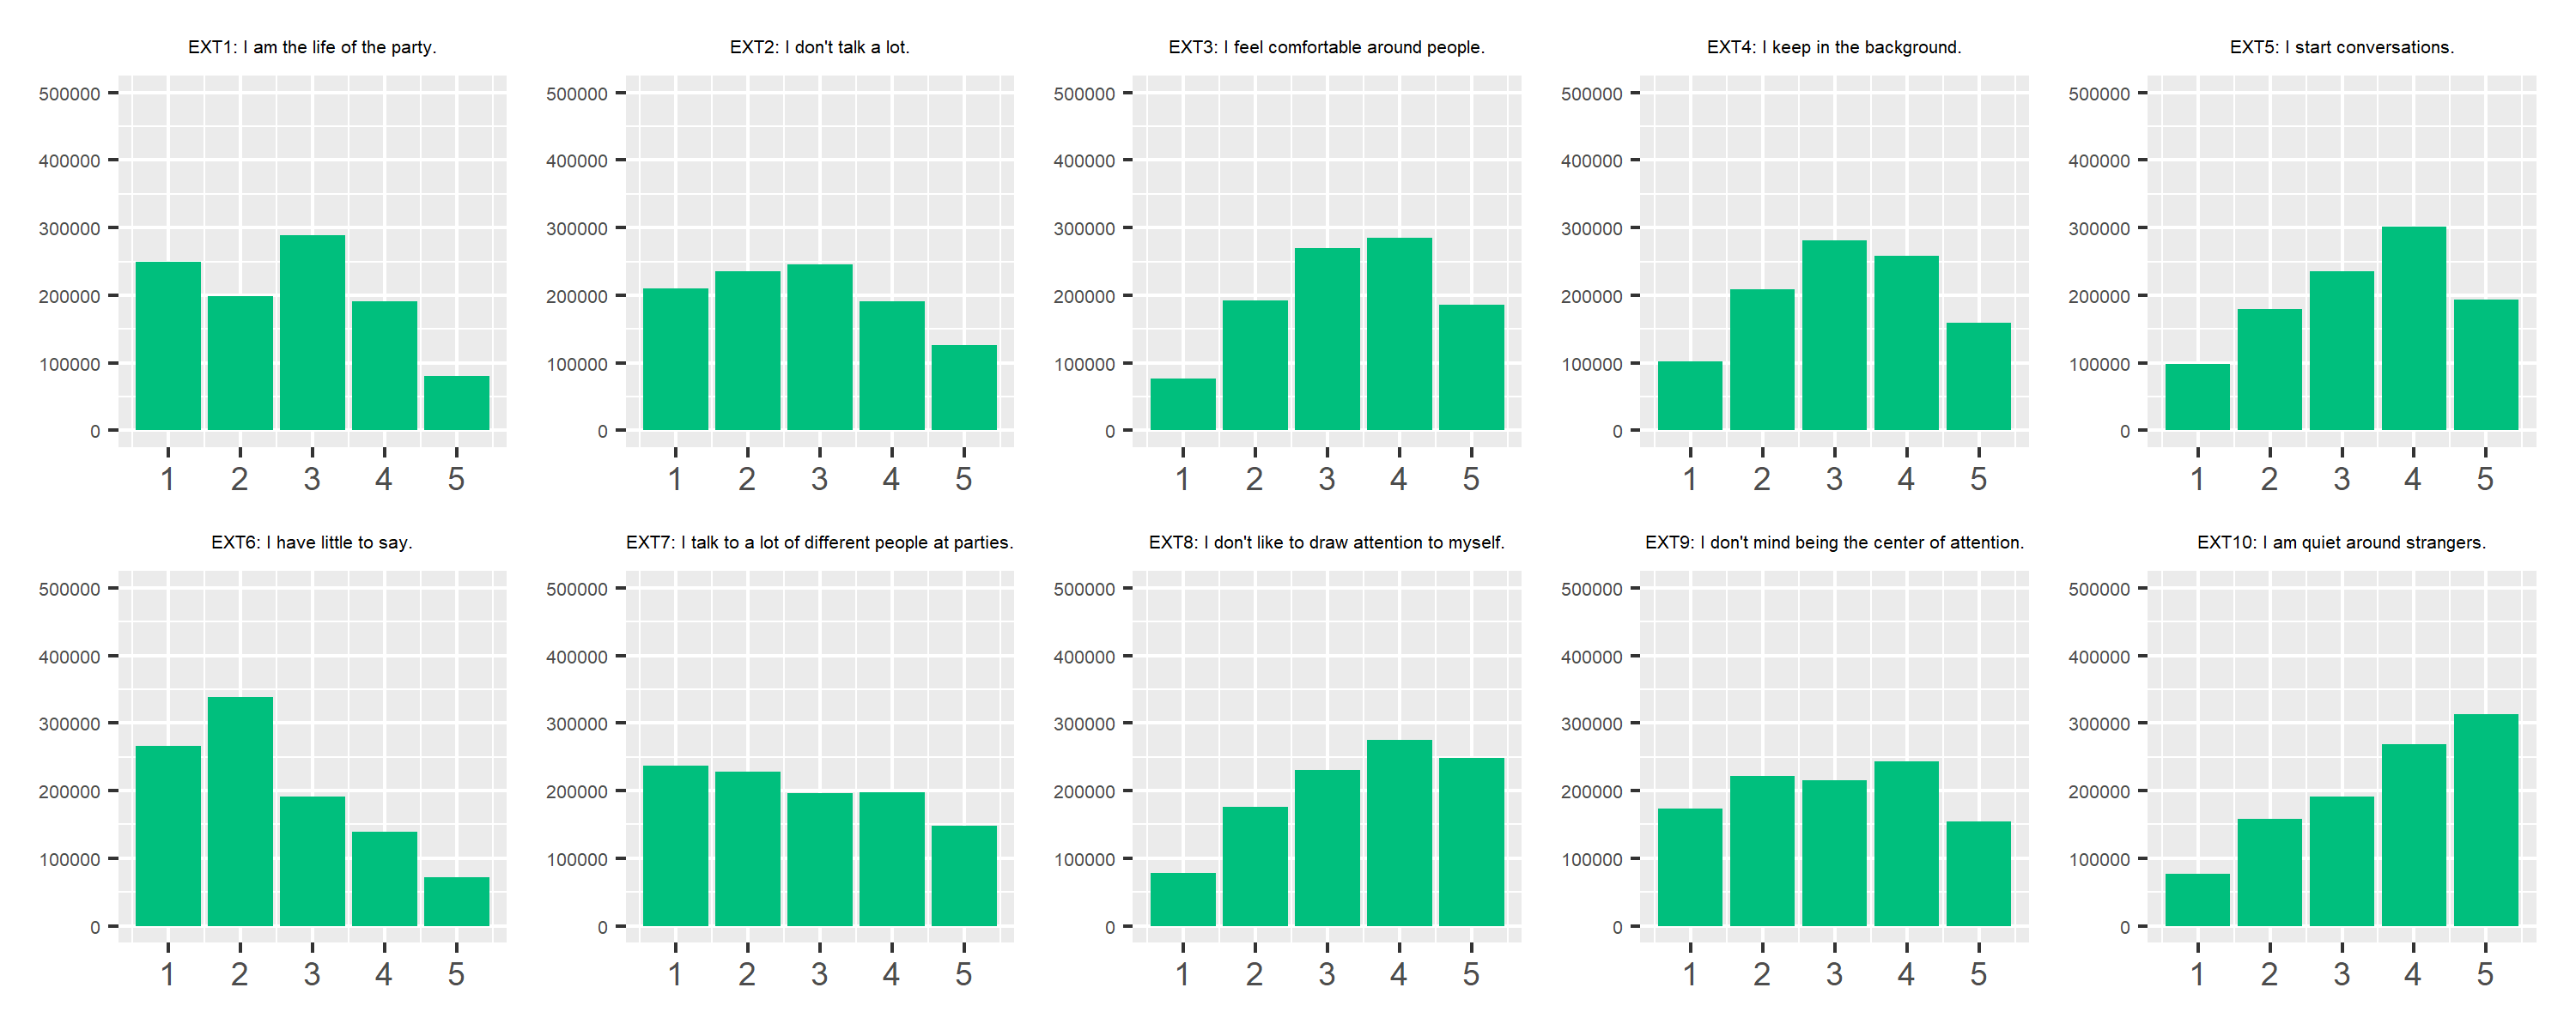
\includegraphics[scale=0.478]{EXT.png}
  \caption{外倾性维度的题目及人数分布}
\end{figure}
\begin{figure}[H]
  \centering
  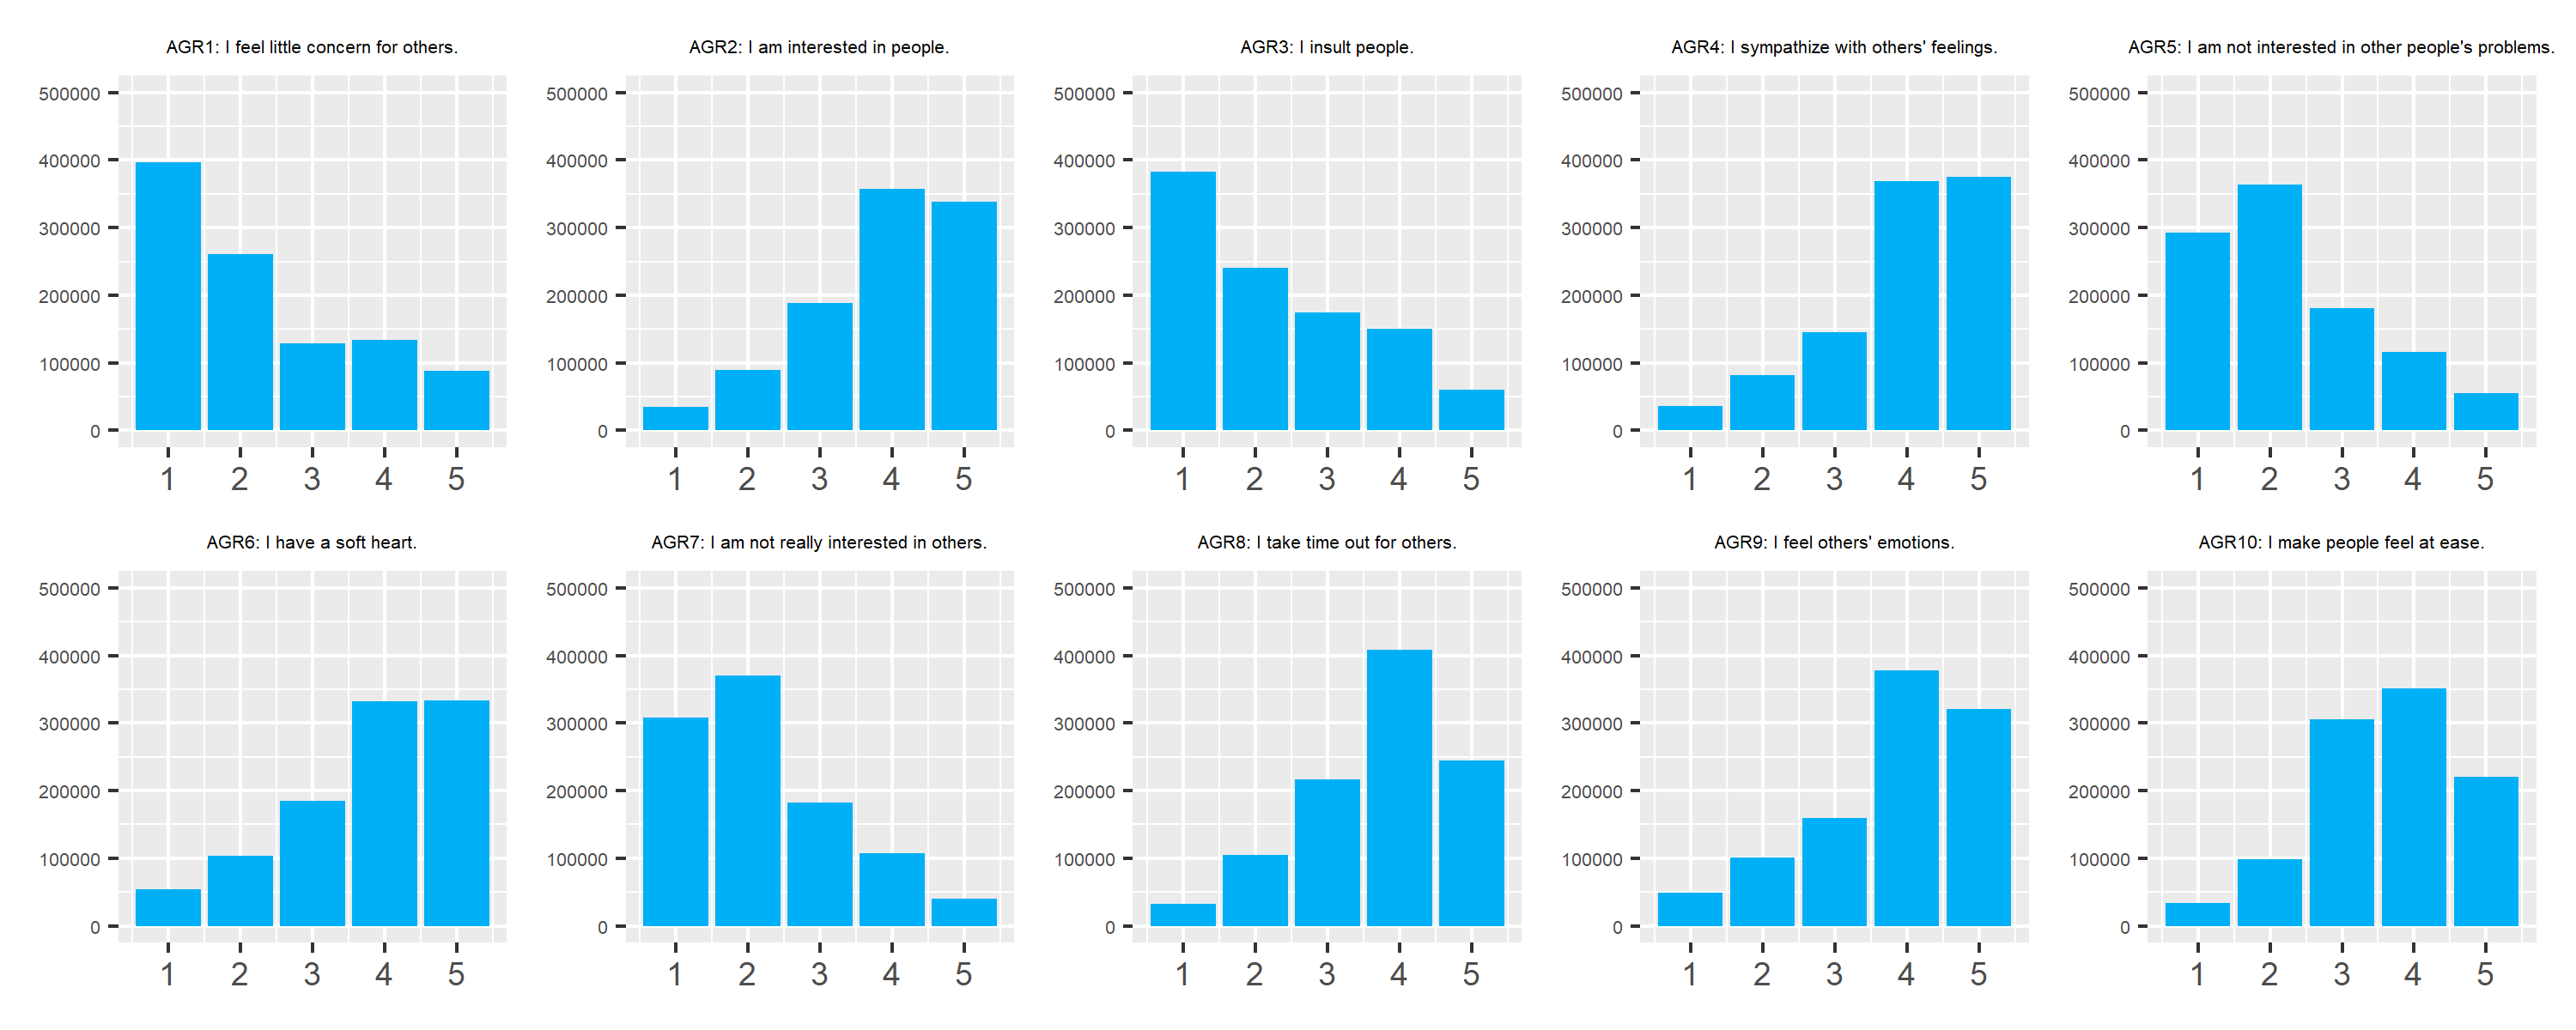
\includegraphics[scale=0.478]{AGR.png}
  \caption{宜人性维度的题目及人数分布}
\end{figure}
\begin{figure}[H]
  \centering
  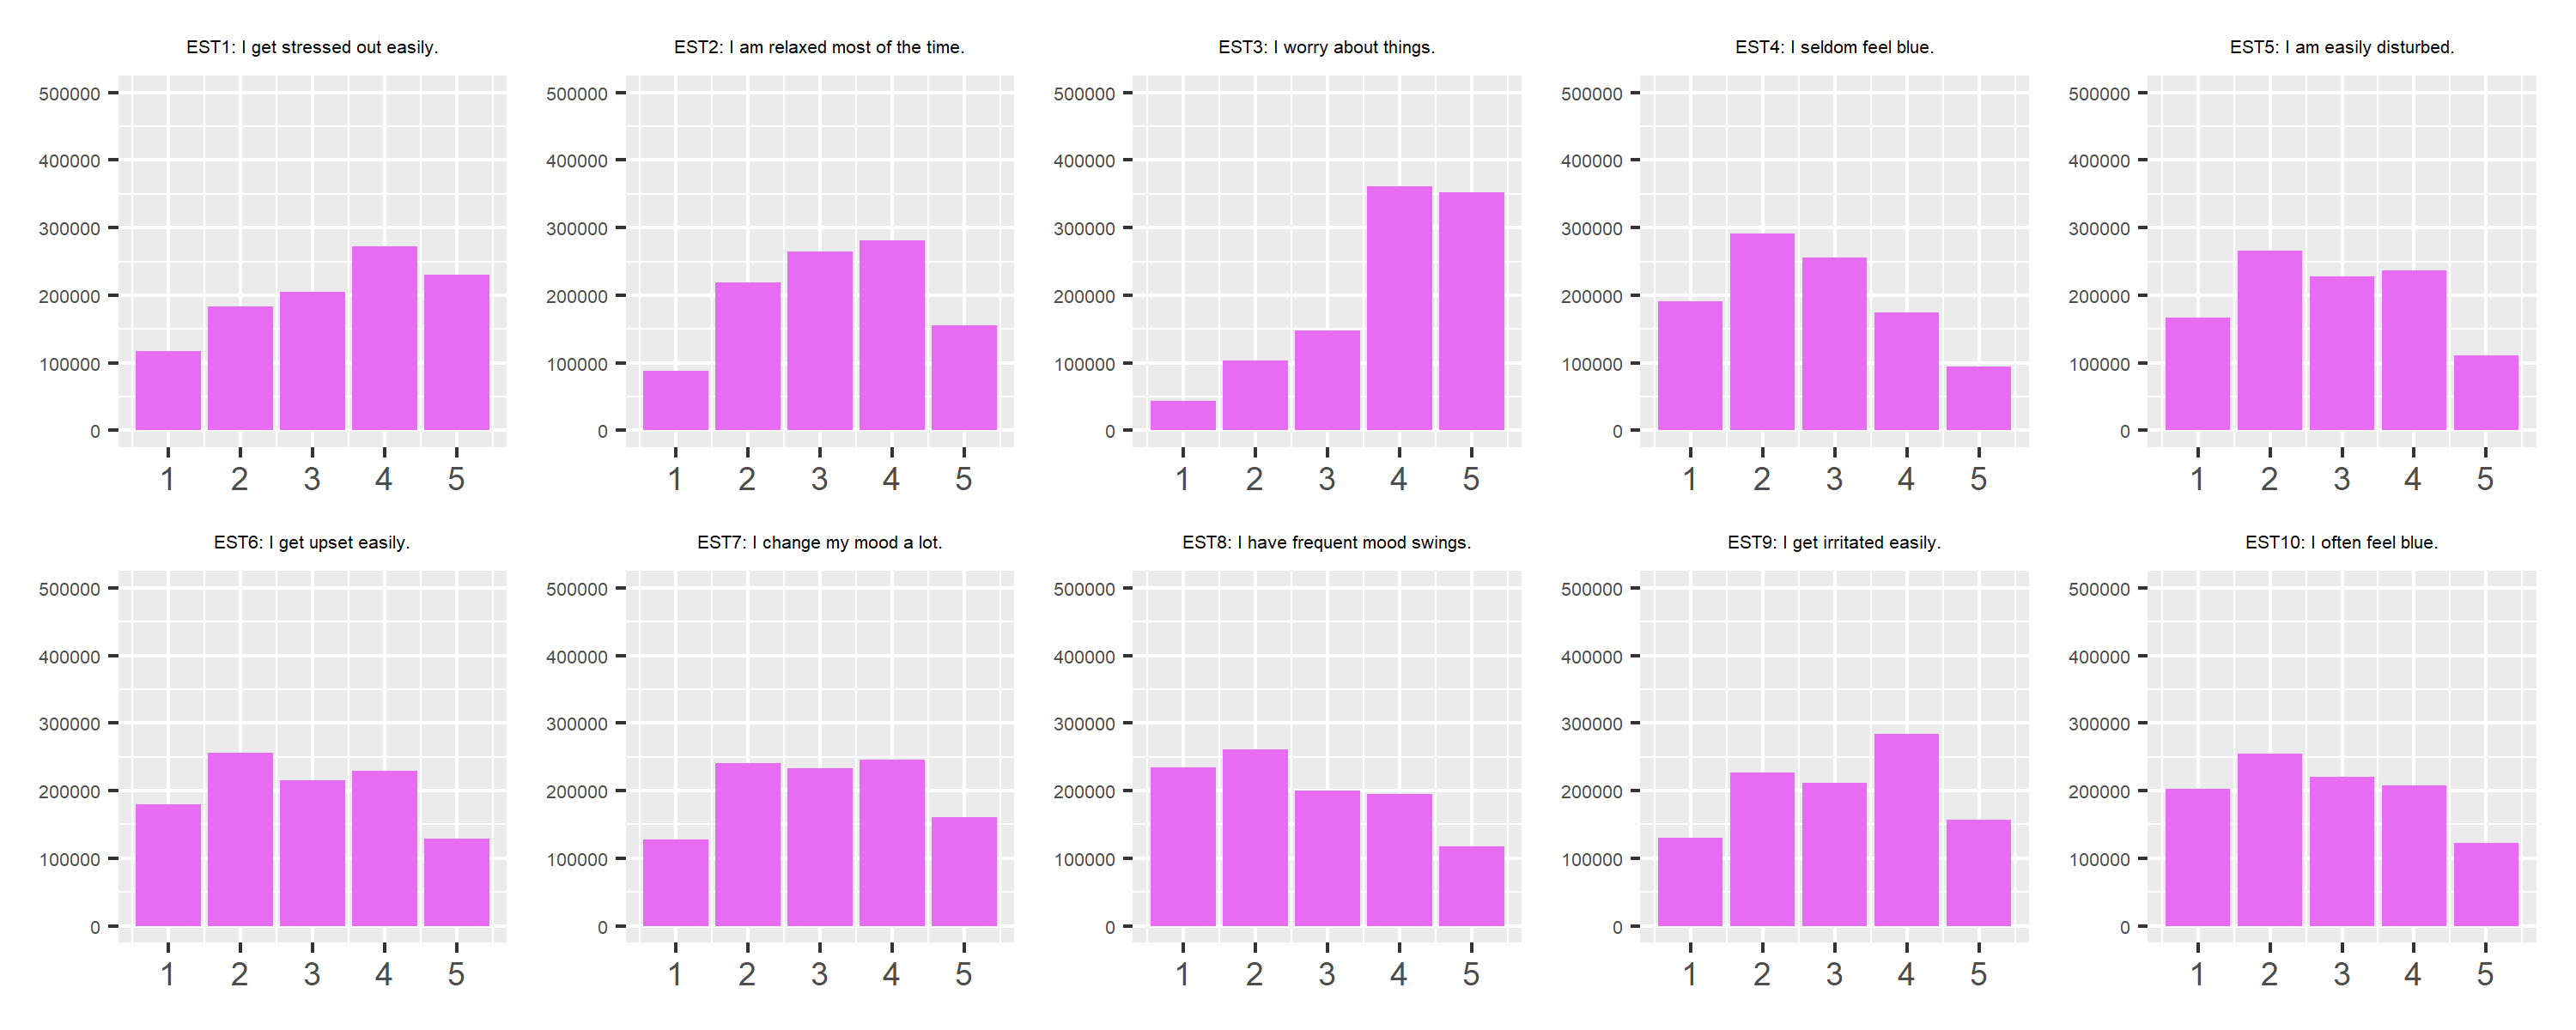
\includegraphics[scale=0.478]{EST.png}
  \caption{情绪性维度的题目及人数分布}
\end{figure}
可以看出,分布图像大致有5种形状:
\begin{itemize}
  \item 单调:按分数1$\sim$5呈单调递增或单调递减,顶部陡峭。
  \item 薄尾:峰值出现在分数2$\sim$4处,并向两侧快速递减,顶部较陡峭。
  \item 厚尾:峰值出现在分数2$\sim$4处,并向两侧缓慢递减,顶部较平坦。
  \item 平顶:分数在1$\sim$5中大约平均分布。
  \item 双峰:在分数1$\sim$2和4$\sim$5中各有一个峰值,整体较平缓。
\end{itemize}
整理出所有题目以及分布类型的对照表如下:
\begin{longtable}{c|c|c}
  \hline
  \textbf{变量名} & \textbf{题目}                                              & \textbf{分布类型} \\\hline
  OPN1         & I have a rich vocabulary.                                & 薄尾            \\\hline
  OPN2         & I have difficulty understanding abstract ideas.          & 单调            \\\hline
  OPN3         & I have a vivid imagination.                              & 单调            \\\hline
  OPN4         & I am not interested in abstract ideas.                   & 单调            \\\hline
  OPN5         & I have excellent ideas.                                  & 薄尾            \\\hline
  OPN6         & I do not have a good imagination.                        & 单调            \\\hline
  OPN7         & I am quick to understand things.                         & 薄尾            \\\hline
  OPN8         & I use difficult words.                                   & 厚尾            \\\hline
  OPN9         & I spend time reflecting on things.                       & 单调            \\\hline
  OPN10        & I am full of ideas.                                      & 单调            \\\hline
  CSN1         & I am always prepared.                                    & 厚尾            \\\hline
  CSN2         & I leave my belongings around.                            & 平顶            \\\hline
  CSN3         & I pay attention to details.                              & 薄尾            \\\hline
  CSN4         & I make a mess of things.                                 & 厚尾            \\\hline
  CSN5         & I get chores done right away.                            & 厚尾            \\\hline
  CSN6         & I often forget to put things back in their proper place. & 双峰            \\\hline
  CSN7         & I like order.                                            & 薄尾            \\\hline
  CSN8         & I shirk my duties.                                       & 厚尾            \\\hline
  CSN9         & I follow a schedule.                                     & 厚尾            \\\hline
  CSN10        & I am exacting in my work.                                & 薄尾            \\\hline
  EXT1         & I am the life of the party.                              & 双峰            \\\hline
  EXT2         & I don't talk a lot.                                      & 厚尾            \\\hline
  EXT3         & I feel comfortable around people.                        & 厚尾            \\\hline
  EXT4         & I keep in the background.                                & 厚尾            \\\hline
  EXT5         & I start conversations.                                   & 厚尾            \\\hline
  EXT6         & I have little to say.                                    & 薄尾            \\\hline
  EXT7         & I talk to a lot of different people at parties.          & 平顶            \\\hline
  EXT8         & I don't like to draw attention to myself.                & 厚尾            \\\hline
  EXT9         & I don't mind being the center of attention.              & 平顶            \\\hline
  EXT10        & I am quiet around strangers.                             & 单调            \\\hline
  AGR1         & I feel little concern for others.                        & 单调            \\\hline
  AGR2         & I am interested in people.                               & 薄尾            \\\hline
  AGR3         & I insult people.                                         & 单调            \\\hline
  AGR4         & I sympathize with others' feelings.                      & 单调            \\\hline
  AGR5         & I am not interested in other people's problems.          & 薄尾            \\\hline
  AGR6         & I have a soft heart.                                     & 单调            \\\hline
  AGR7         & I am not really interested in others.                    & 薄尾            \\\hline
  AGR8         & I take time out for others.                              & 薄尾            \\\hline
  AGR9         & I feel others' emotions.                                 & 薄尾            \\\hline
  AGR10        & I make people feel at ease.                              & 薄尾            \\\hline
  EST1         & I get stressed out easily.                               & 厚尾            \\\hline
  EST2         & I am relaxed most of the time.                           & 厚尾            \\\hline
  EST3         & I worry about things.                                    & 薄尾            \\\hline
  EST4         & I seldom feel blue.                                      & 厚尾            \\\hline
  EST5         & I am easily disturbed.                                   & 双峰            \\\hline
  EST6         & I get upset easily.                                      & 双峰            \\\hline
  EST7         & I change my mood a lot.                                  & 平顶            \\\hline
  EST8         & I have frequent mood swings.                             & 厚尾            \\\hline
  EST9         & I get irritated easily.                                  & 双峰            \\\hline
  EST10        & I often feel blue.                                       & 厚尾            \\\hline
  \caption{题目及人数分布类型}
  \label{type}
\end{longtable}
其中,仅厚尾、平顶和双峰形状可近似看成测试者集中于中间分数,单调和薄尾形状的测试者均严重偏向于两端分数,
二者的比例恰好为$1:1$。这说明在相当一部分题目中,参加测验的人会更倾向于极端的态度。
此外,题目的分布类型在不同的维度也有各自的特点:
\begin{itemize}
  \item 开放性维度题目的分布类型为单调和薄尾,人数分布差异很大。
  \item 尽责性维度题目的分布类型多为厚尾和薄尾,人数分布比较均匀。
  \item 外倾性维度题目的分布类型多为厚尾和平顶,人数分布很均匀。
  \item 宜人性维度题目的分布类型为薄尾和单调,人数分布差异很大。
  \item 情绪性维度题目的分布类型多为厚尾和双峰,人数分布很均匀。
\end{itemize}
在同一维度下题目中,假如大多数人都同样有高分或低分倾向,那么他们的人格特质在这个维度上的区分度不会太高;
假如所有人均匀分布在每个分数上,那么也许可以根据分数的差异,划分出具有不同人格特质的人群。
因此,尽责性、外倾性和情绪性可能是体现人格特质差异的主要维度,而开放性和宜人性则是次要维度。
% 一个比较有意思的情况是,不少相近叙述或反向叙述的题目具有不同的分布类型,
% 比如EXT2和EXT6(厚尾和薄尾)、AGR4和AGR9(单调和薄尾)。
% 这说明在改变题目叙述方式后,有相当一部分人的倾向选择也发生了变化。
% 这种变化差异也许就是人们具有人格特质差异的表现,也从侧面体现了题目设置的巧妙之处。
\section{维度和题目的相关性分析}
% 对于一对相近或反向叙述的题目,理应具有比较高的正相关性或负相关性,
% 但是人数分布的图像显示并不完全是这样,即图像不属于同一种形状。
计算各个题目之间的相关系数,画出相关系数矩阵图如下:
\begin{figure}[H]
  \centering
  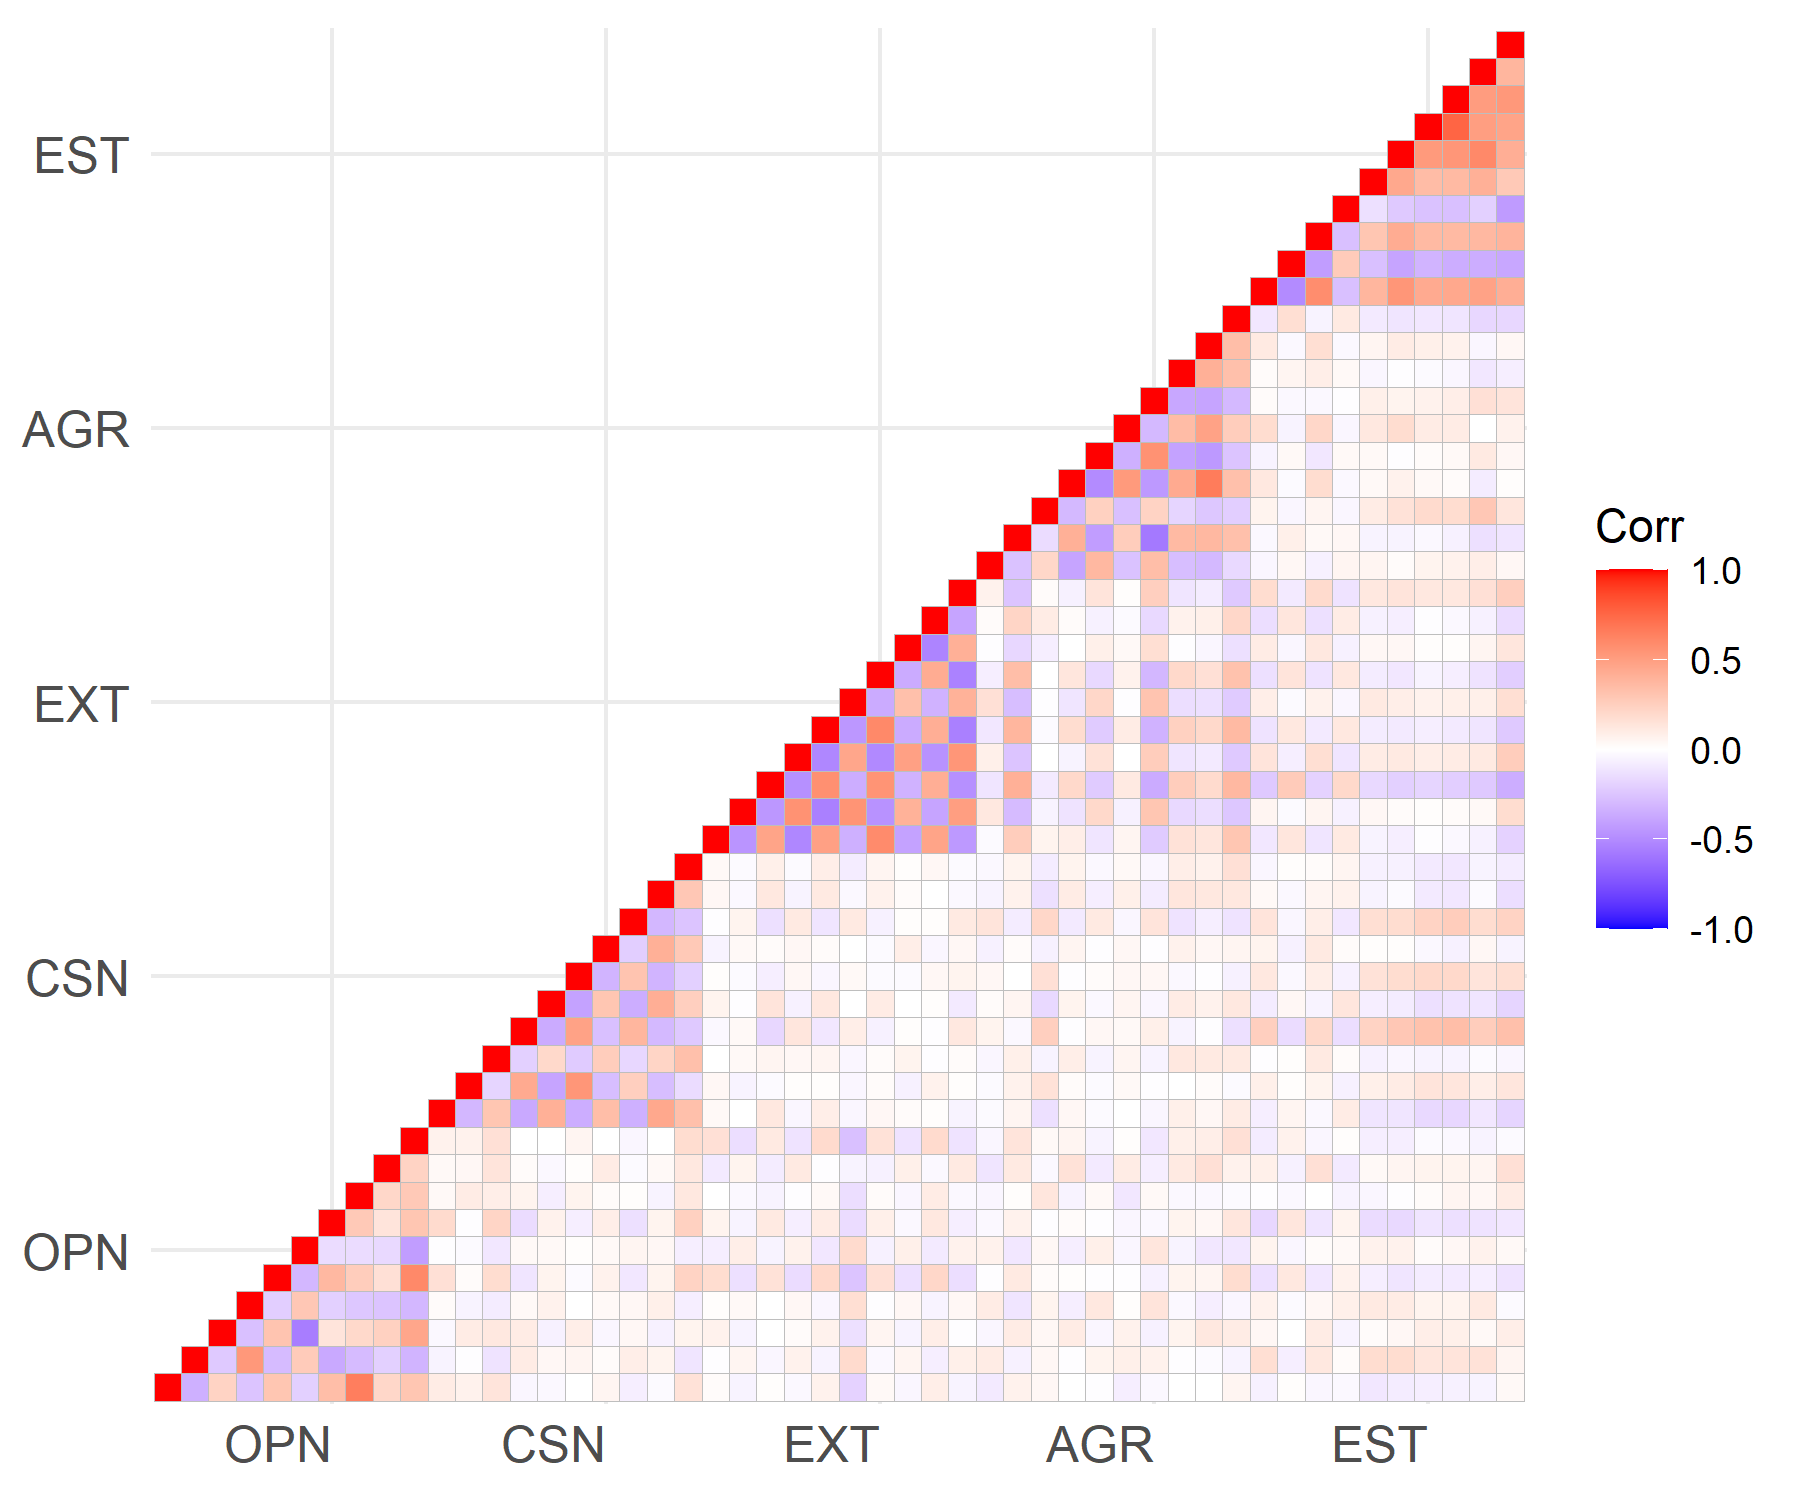
\includegraphics[scale=0.7]{Corrplot_Item.png}
  \caption{题目间的相关系数}
\end{figure}
图像显示,同一维度下的题目具有比较高的相关性,而不同维度的题目相关性较低。
这样的特点支持了用10个题目的总分作为该维度人格倾向的计分方式,
而且维度之间的低相关性表示维度之间重叠较少,5个维度很好地代表了人格特征的5个不同方面。
% 对于前面文字描述上关联性较强的题目,其相关系数分别为:
% \begin{longtable}{c|c|c|c|c}
%   \hline
%   题目&CSN4-CSN6&EXT2-EXT6&AGR4-AGR9&EST6-EST10\\\hline
%   相关系数&0.4810&0.5469&0.6579&0.4241\\\hline
% \end{longtable}
同时发现,外倾性(EXT)和宜人性(AGR)、外倾性(EXT)和情绪性(EST)、
尽责性(CSN)和情绪性(EST)之间的部分题目也存在一定的相关性。\par
% 数据显示部分题目间的相关系数达到$0.4$以上。
将题目分数汇总为维度总分,计算各个维度之间相关系数,画出相关系数矩阵图如下:
\begin{figure}[H]
  \centering
  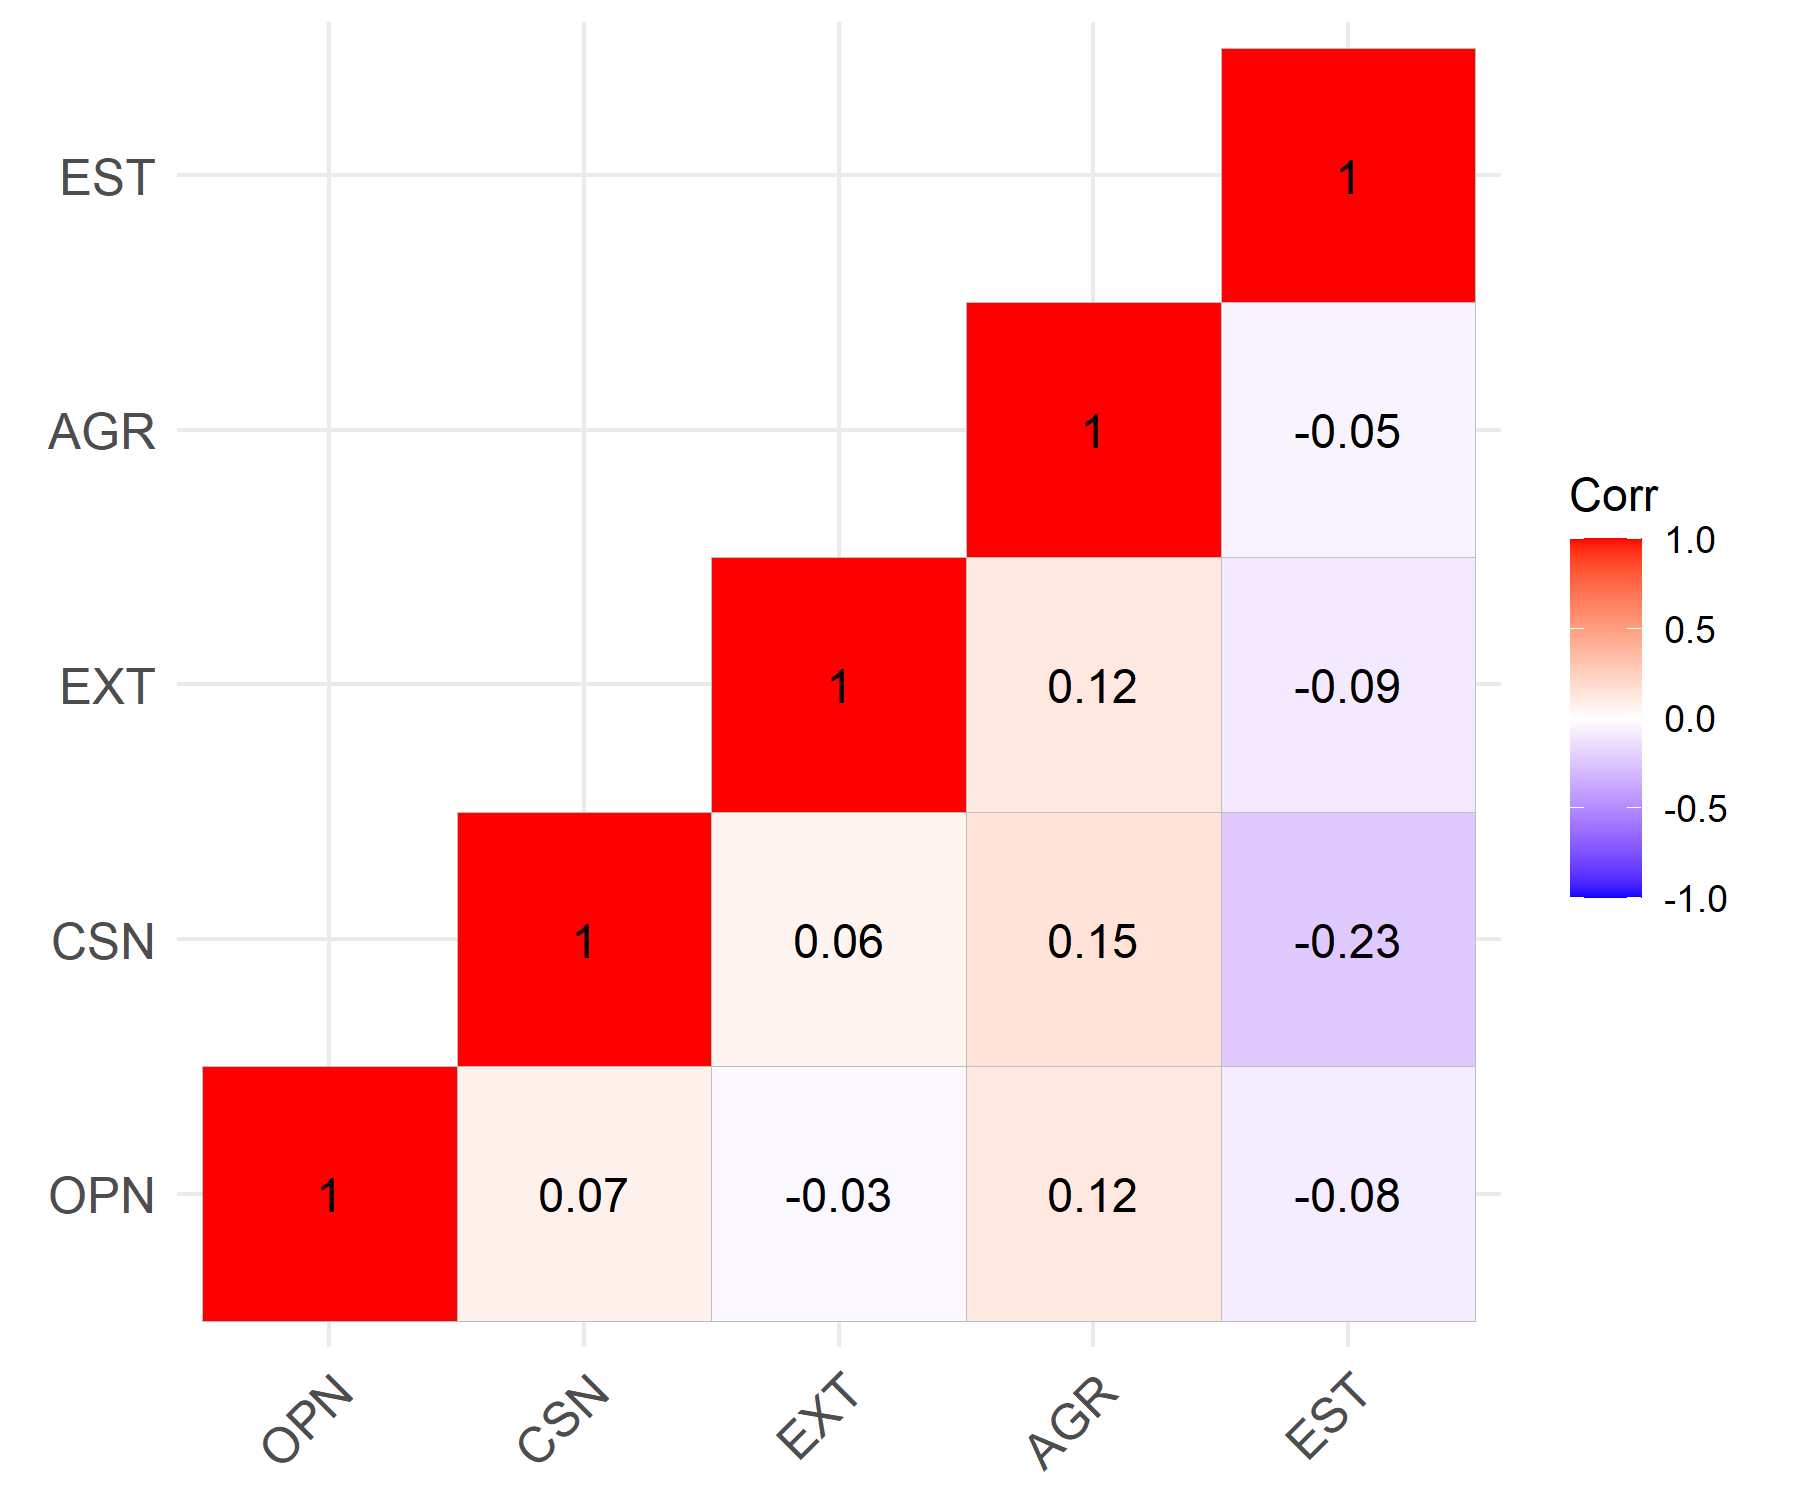
\includegraphics[scale=0.7]{Corrplot_Dimension.png}
  \caption{维度间的相关系数}
\end{figure}
% 将反向记分的题目处理后,计算每个维度下10道题目总分的相关系数,画出相关系数矩阵图。
图像显示,维度之间的相关系数均在一个很低的水平。
其中,尽责性(CSN)和情绪性(EST)是唯一一对相关系数绝对值超过0.2的维度,
一种可能的解释是责任感强的人有更强的抗压能力,更不容易有情绪化反应,因此二者呈微弱的负相关。\par
综上所述,维度内部的题目具有较高相关性,表明10个题目都指向同一个维度。
虽然不同维度之间的题目存在一些低度相关的情况,但维度之间仅存在个别微弱相关,
所以认为5个维度是相互独立的5个方面。
\section{测试者的国家分布}
除去国籍未知的情况,数据中的测试者共来自222个国家,
其中人数超过$10,000$人的国家有12个。
\begin{figure}[H]
  \centering
  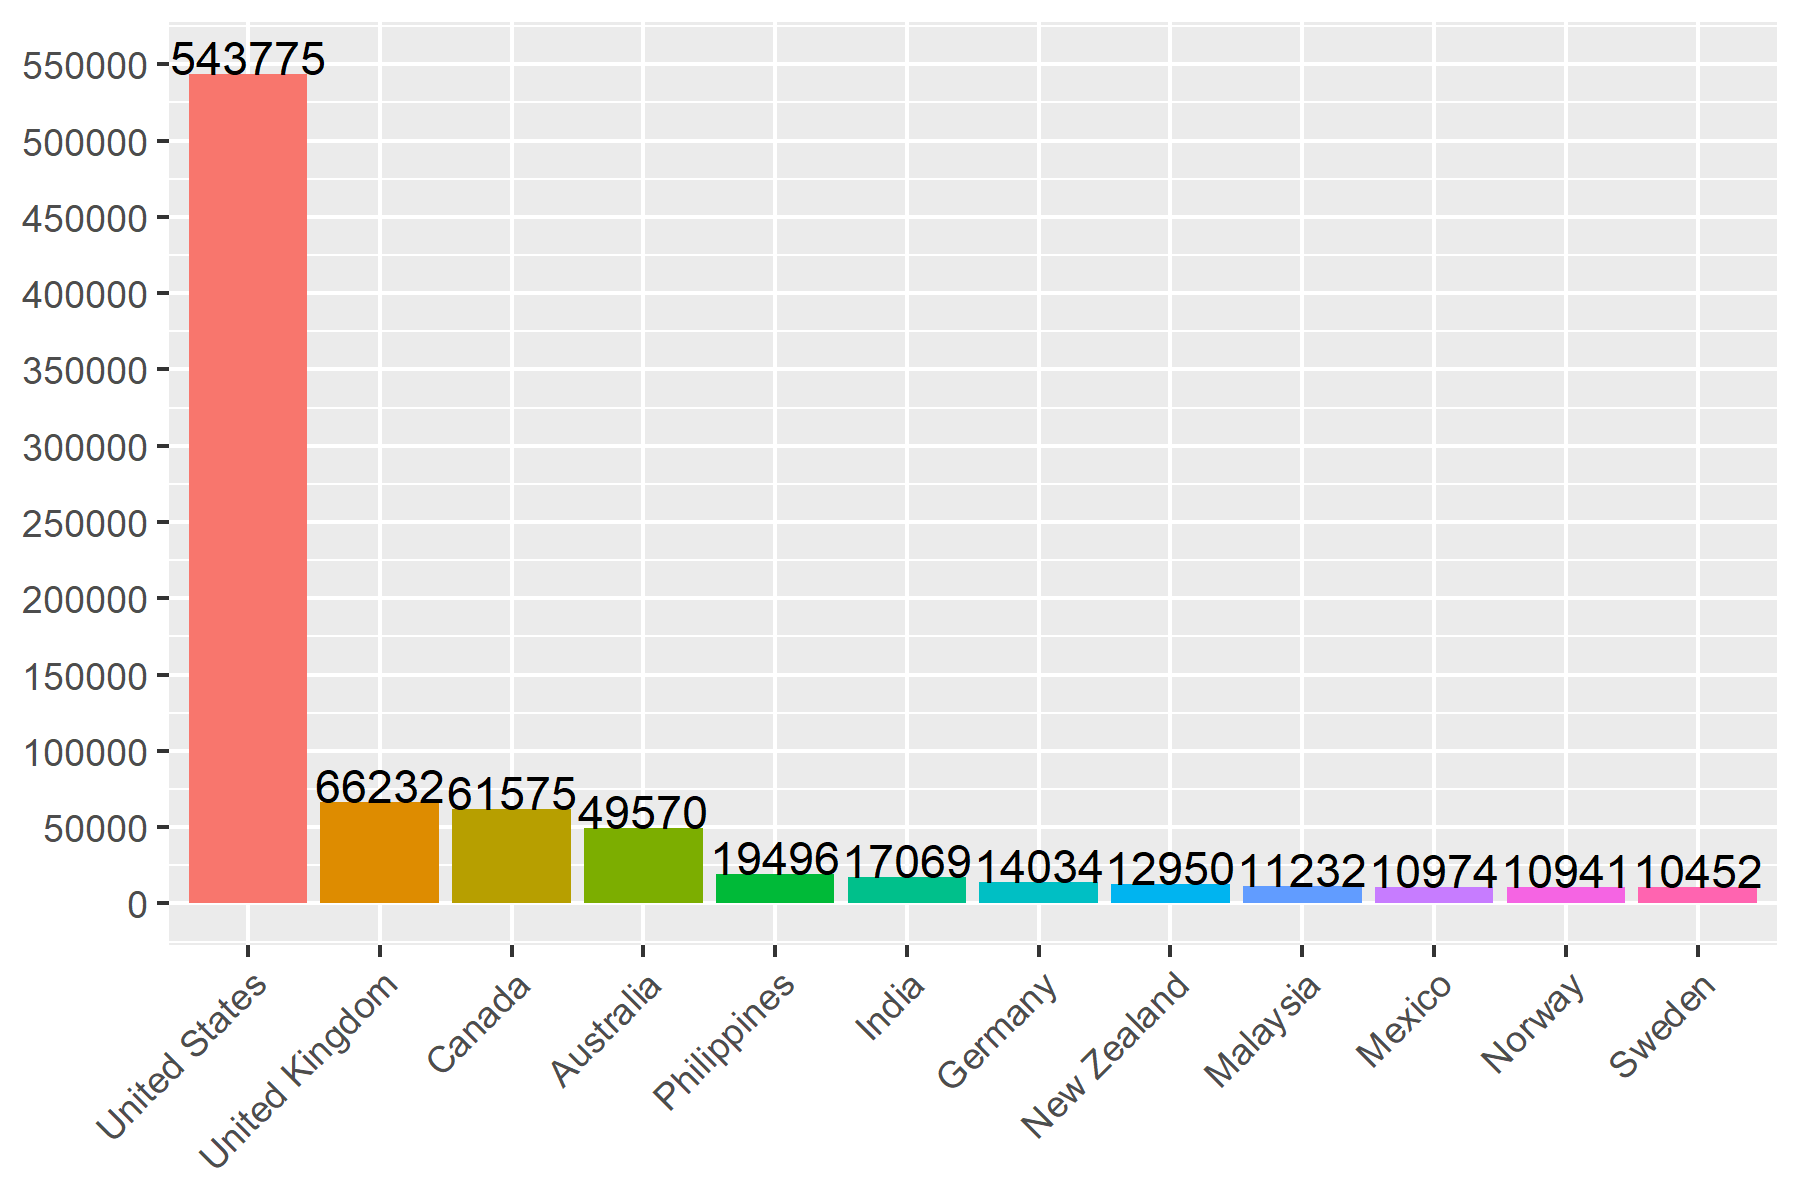
\includegraphics[scale=0.79]{Country.png}
  \caption{参加测验人数超过$10,000$的国家}
\end{figure}
来自美国的测试者占样本数据的一半以上,其余国家的人数均显著小于美国,
同时绝大部分国家的测试者不足$10,000$人。
% 如果以平均倾向得分代表该国的人格特质倾向,那么该数据对于美国人的特质倾向将是比较好的研究材料,
% 研究其他参加者较少的国家时可能会因为样本量较少而出现偏差。
% 因此,在比较国家之间的人格特质差异时,将主要针对参加者人数较多的国家,人数较少的国家结果仅供参考。
因此,该数据不宜作为研究国家之间人格特质差异的材料,但就研究人类群体的人格特质来说,
该数据足够概括大部分情况。
\part{维度与分布类型的独立性检验}
% \setcounter{section}{0}
% \section{人数分布类型统计}
根据表\ref{type}可知,题目分布的类型在各维度中并不是随机出现的,每个维度都有各自的分布特点。
统计每个维度中不同分布类型的个数,得到下表:
\begin{longtable}{c|c|c|c|c|c}
  \hline
  维度  & 单调 & 薄尾 & 厚尾 & 平顶 & 双峰 \\\hline
  OPN & 6  & 3  & 1  & 0  & 0  \\
  CSN & 0  & 3  & 5  & 1  & 1  \\
  EXT & 1  & 1  & 5  & 2  & 1  \\
  AGR & 4  & 6  & 0  & 0  & 0  \\
  EST & 0  & 1  & 5  & 1  & 3  \\\hline
  \caption{维度与分布类型列联表}
\end{longtable}
为了研究维度与分布类型是否有联系,对其进行卡方独立性检验。
由于表中部分单元格数值太小,直接计算出卡方统计量很可能不准确,
采用2000次蒙特卡罗模拟的数据,卡方检验结果如下:
\begin{longtable}{c|c}
  \hline
  X-squared & 36.341   \\\hline
  p-value   & 0.000995 \\\hline
  \caption{维度与分布类型的卡方独立性检验(基于2000次蒙特卡罗模拟)}
\end{longtable}
因为p值相当小,认为维度与题目的分布类型不是相互独立的。
测试者在不同维度下题目的分布类型不同,说明人们在5个维度上并不全是以中立态度为为中心的对称分布。
在开放性维度和宜人性维度,人们普遍表现为高分倾向;
而在尽责性维度、外倾性维度和情绪性维度,人们在不同倾向间分布较为平均。
% 说明5个维度的人格特质在构成完整的人格时,各自的作用相互独立,
% 5个维度分别代表人格的5个不同方面,5个方面构成一个人的完整人格。
\part{关于Big5人格测验结果的聚类分析}
\setcounter{section}{0}
\section{聚类方法}
数据中的分数1$\sim$5表示题目对测试者来说的符合程度,那么分数的差异可以理解为题目符合程度的差异;
同理,维度总分的差异就是该维度上人格特质的差异。
人格的构成并不仅仅是特质倾向的简单排列组合,对比“类型说”的人格测验,
也许会有几种具有固定特质倾向的典型人格,表现为相近的维度总分。
我们可以基于5个维度总分对测试者的人格聚类,研究能够提取出多少种典型人格,以及他们各自的倾向性特征,
进而了解每个维度在区分不同人格时的重要性。\par
% 将维度总分相近的样品划分为同一类,
% 聚类的结果实现了从“特质倾向分数”到“特定人格类型”的转换,
% 可以给出更为直观的特质展示,
% 也可以和“类型说”测验的特定人格类型作比较。
在对大样本数据进行聚类分析时,K-均值聚类方法聚类速度快、效果好,因此选用K-均值聚类方法。
首先随机选K个点作为初始类中心,然后逐渐把周围的点分配到与类中心最近的类中,
每次有新的点加入到类中都需要重新计算类均值,重复分配点和计算类均值的过程,
直到各类都没有新的点加入或移出,最后得到K个类的聚类结果。\par
% 在处理过反向记分题目的数值后,将各个维度下的分数加总得到维度总分,以5个维度总分作为聚类的样本数据。
% 维度总分的取值范围为10$\sim$50,将其标准化
% \begin{equation}
%   Dim\_scale = \frac{Dim\_total-30}{20}
% \end{equation}
% 使其取值范围变为-1$\sim$1。
聚类计算过程在\texttt{R}中进行。
\section{设置超参数}
\subsection*{类的个数}
聚类的个数不能太少,也不能太多,否则会失去实际意义。
因为Big5人格测验的特质维度是5,所以类的个数不能少于5。
以0为临界点,将用公式\ref{scale}标准化后的维度总分$DimScore\_scale$分为两部分,
$DimScore\_scale<0$表示低分倾向,$DimScore\_scale>0$表示高分倾向,则5个维度共有32种倾向组合。
综上所述,将类的个数限定在5$\sim$32个。\par
使用\texttt{NbClust}包的\texttt{NbClust}函数确定最优类的个数,测度距离采用欧氏距离,
设置最小类的个数为5,最大类的个数为32。
\texttt{NbClust}函数会计算出多个用于判断类的个数的指标,以投票的方式确定一个最优个数。
\subsection*{$Bagging$方法}
由于算力的限制,无法把全部数据导入\texttt{NbClust}函数,采用$Bagging$方法减少单次计算使用的数据量。\par
从样本中随机抽取$1,000$个样品,用于\texttt{NbClust}函数计算最优的类个数,
重复10次,确定最优类的个数如下:
\begin{longtable}{c|cccccccccc}
  \hline
  样本编号  & 1 & 2 & 3 & 4 & 5 & 6 & 7 & 8 & 9 & 10 \\\hline
  最优类个数 & 5 & 5 & 5 & 5 & 5 & 5 & 5 & 5 & 6 & 5  \\\hline
  \caption{$Bagging$方法确定最优类的个数}
\end{longtable}
显然,认为最优的聚类个数为5,因此使用5-均值聚类方法进行聚类分析。
\section{聚类结果展示}
使用\texttt{biganalytics}包的\texttt{bigkmeans}函数进行大数据5-均值聚类。
迭代收敛后,5个类的分别为:
\begin{longtable}{c|c|c}
  \hline
  % 类编号   & 1        & 2        & 3        & 4        & 5        \\\hline
  % 样品数   & 206591   & 204976   & 268242   & 139360   & 189021   \\\hline
  % 类内平方和 & 55730.16 & 61333.91 & 79960.60 & 56904.41 & 60890.40 \\\hline
  类编号 & 样品数    & 类内平方和    \\\hline
  1   & 206591 & 55730.16 \\\hline
  2   & 204976 & 61333.91 \\\hline
  3   & 268242 & 79960.60 \\\hline
  4   & 139360 & 56904.41 \\\hline
  5   & 189021 & 60890.40 \\\hline
  \caption{5-均值聚类结果}
\end{longtable}
其中每个类的样品数差距不大,类内平方和也都在同一水平。类的中心分别为:
\begin{longtable}{c|c|c|c|c|c}
  \hline
  类编号 & OPN   & CSN   & EXT   & AGR   & EST   \\\hline
  1   & 40.08 & 39.28 & 30.56 & 41.10 & 36.12 \\\hline
  2   & 41.61 & 26.00 & 30.00 & 39.24 & 37.69 \\\hline
  3   & 40.38 & 37.30 & 31.01 & 41.92 & 21.60 \\\hline
  4   & 41.39 & 33.41 & 29.80 & 26.90 & 26.45 \\\hline
  5   & 30.67 & 30.70 & 30.43 & 34.46 & 33.23 \\\hline
  \caption{5-均值聚类中心}
  \label{center}
\end{longtable}
% \noindent 类的中心代表了该类样品的平均维度总分。
\noindent 将每个类的分布表现在条形图上:
\begin{figure}[H]
  \centering
  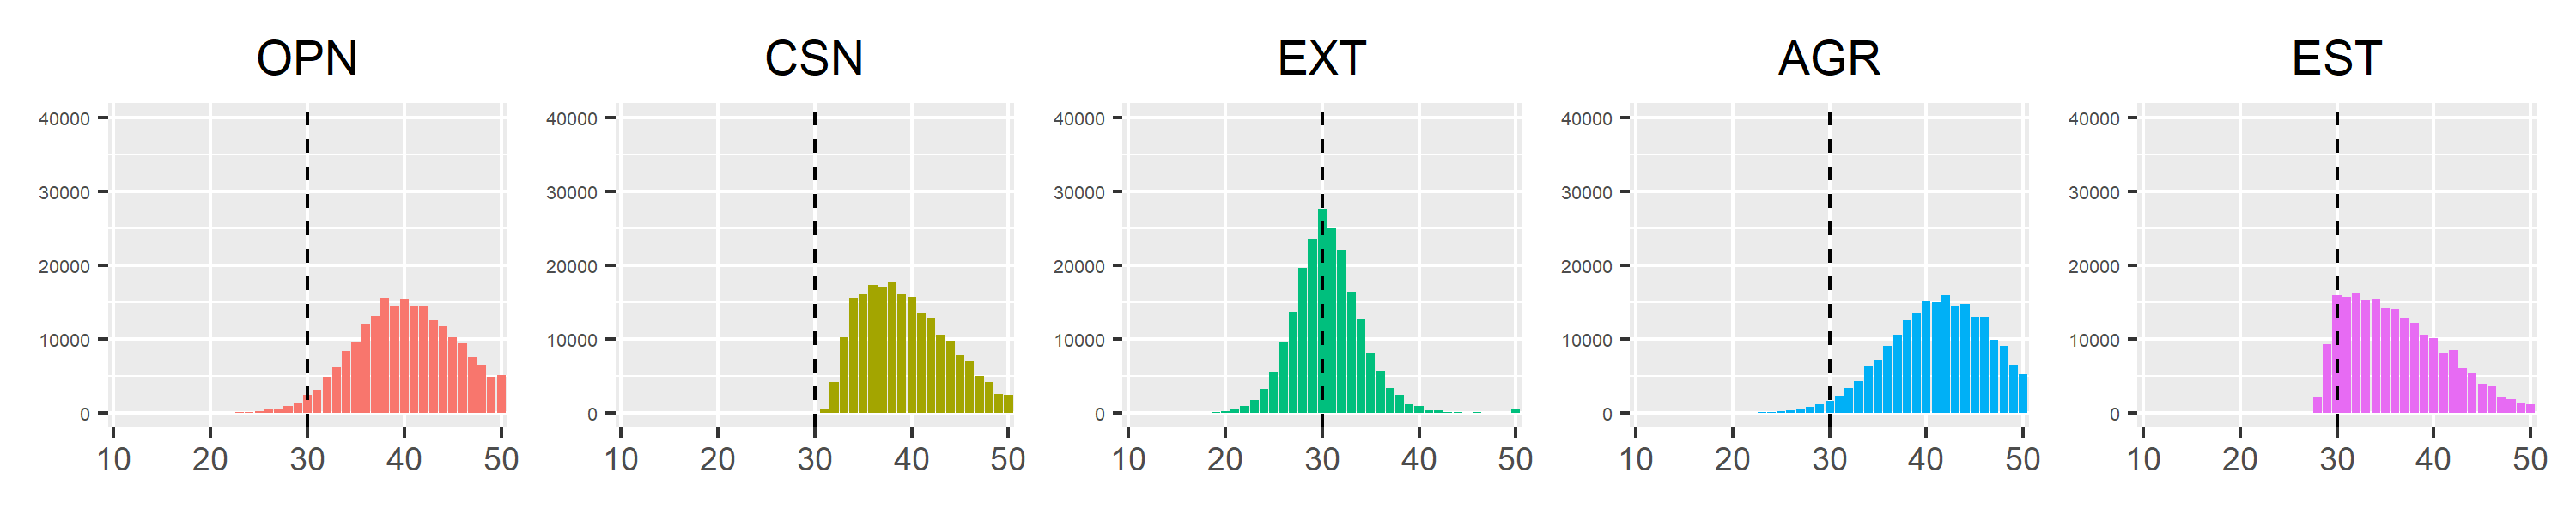
\includegraphics[scale=0.478]{Cluster1.png}
  \caption{类1(206591个样品)的分布}
\end{figure}
\begin{figure}[H]
  \centering
  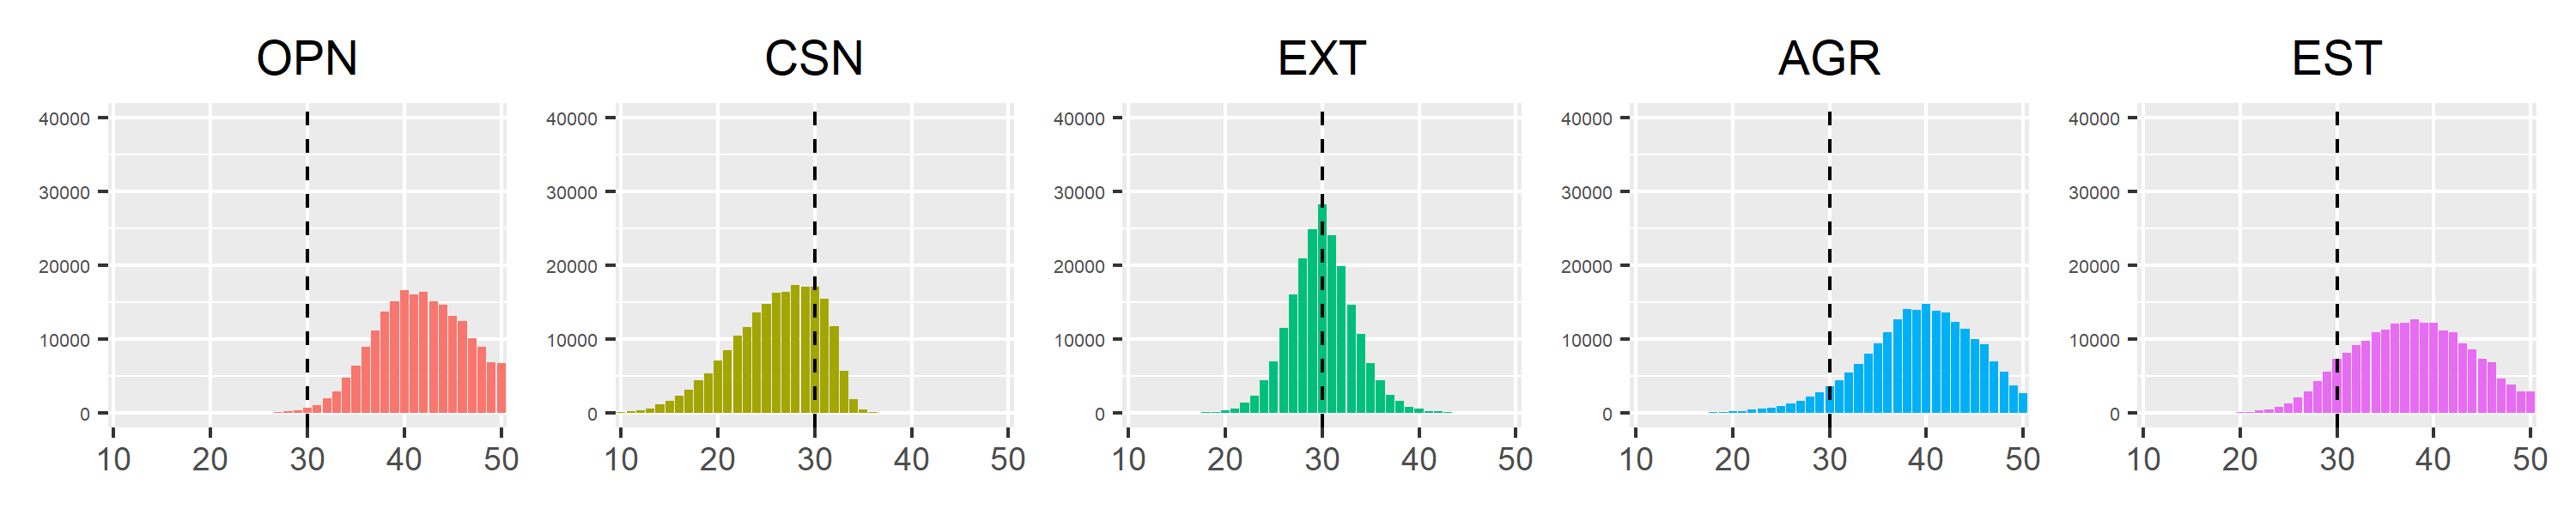
\includegraphics[scale=0.478]{Cluster2.png}
  \caption{类1(204976个样品)的分布}
\end{figure}
\begin{figure}[H]
  \centering
  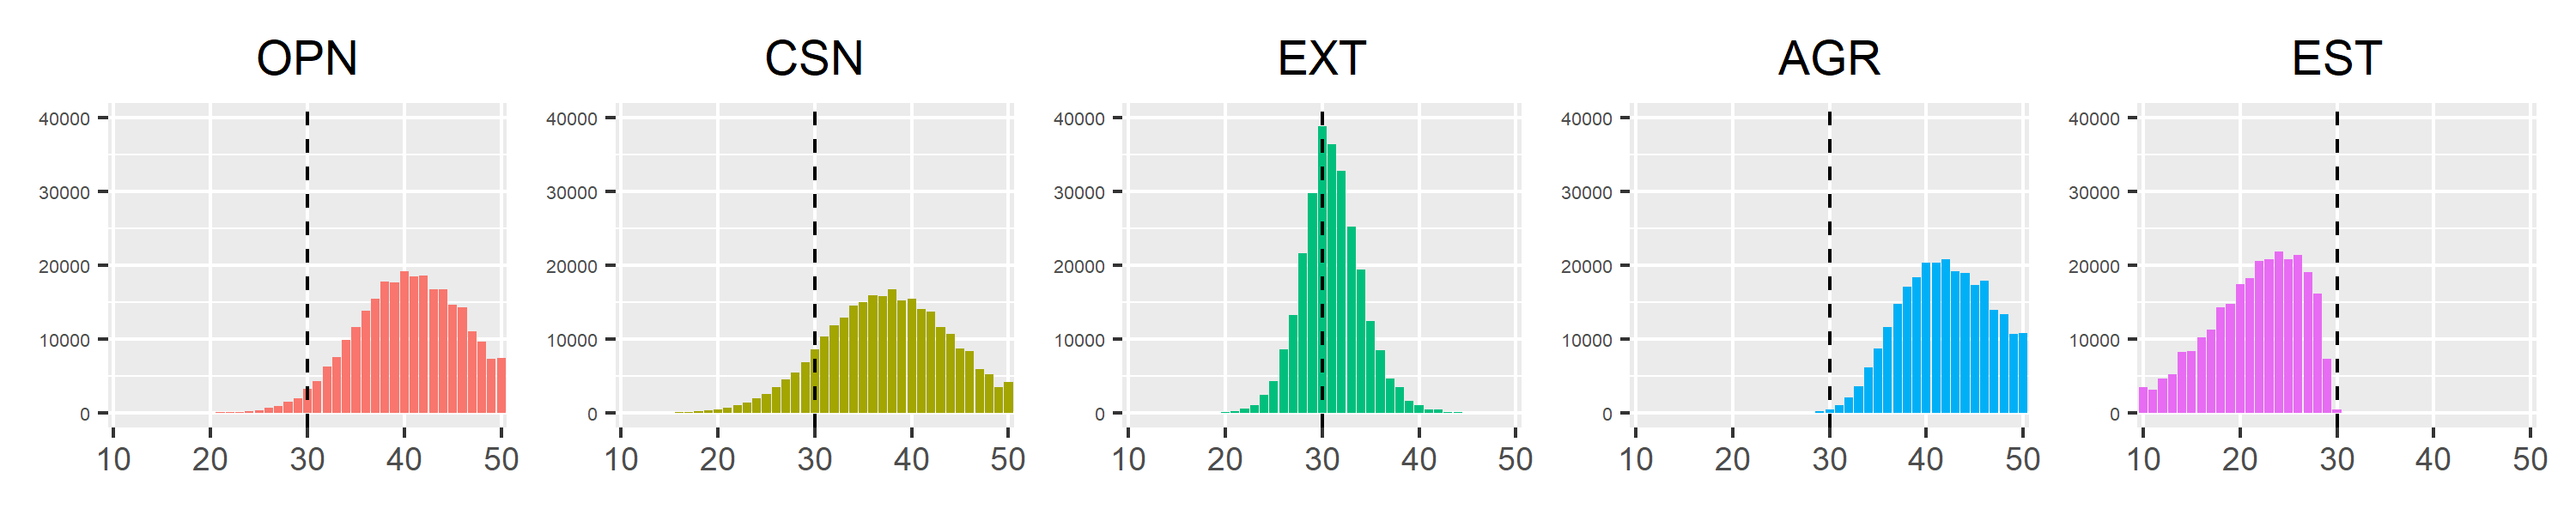
\includegraphics[scale=0.478]{Cluster3.png}
  \caption{类1(268242个样品)的分布}
\end{figure}
\begin{figure}[H]
  \centering
  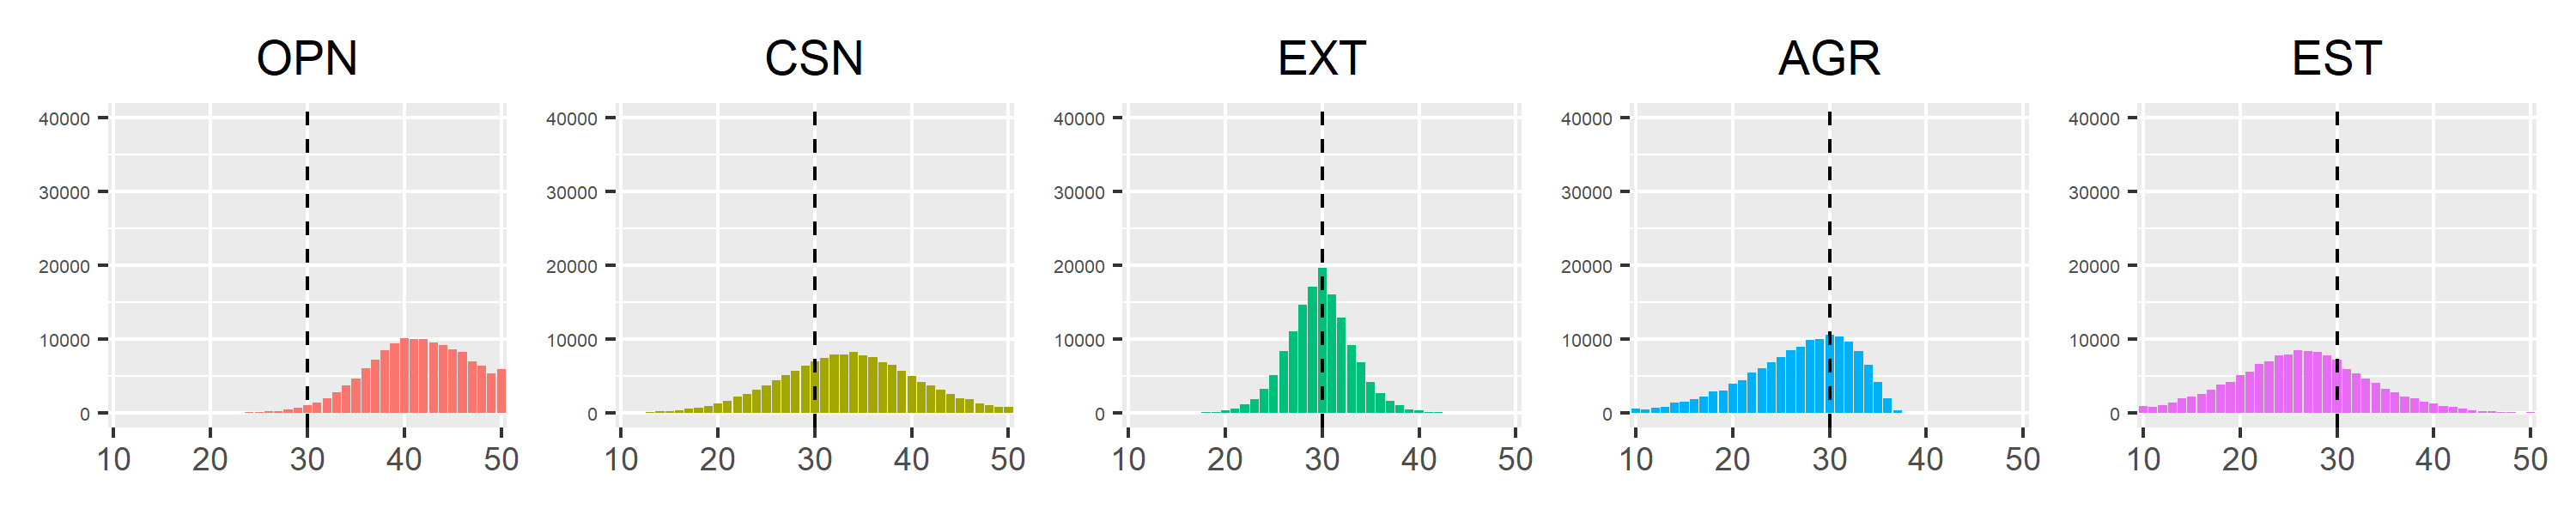
\includegraphics[scale=0.478]{Cluster4.png}
  \caption{类1(139360个样品)的分布}
\end{figure}
\begin{figure}[H]
  \centering
  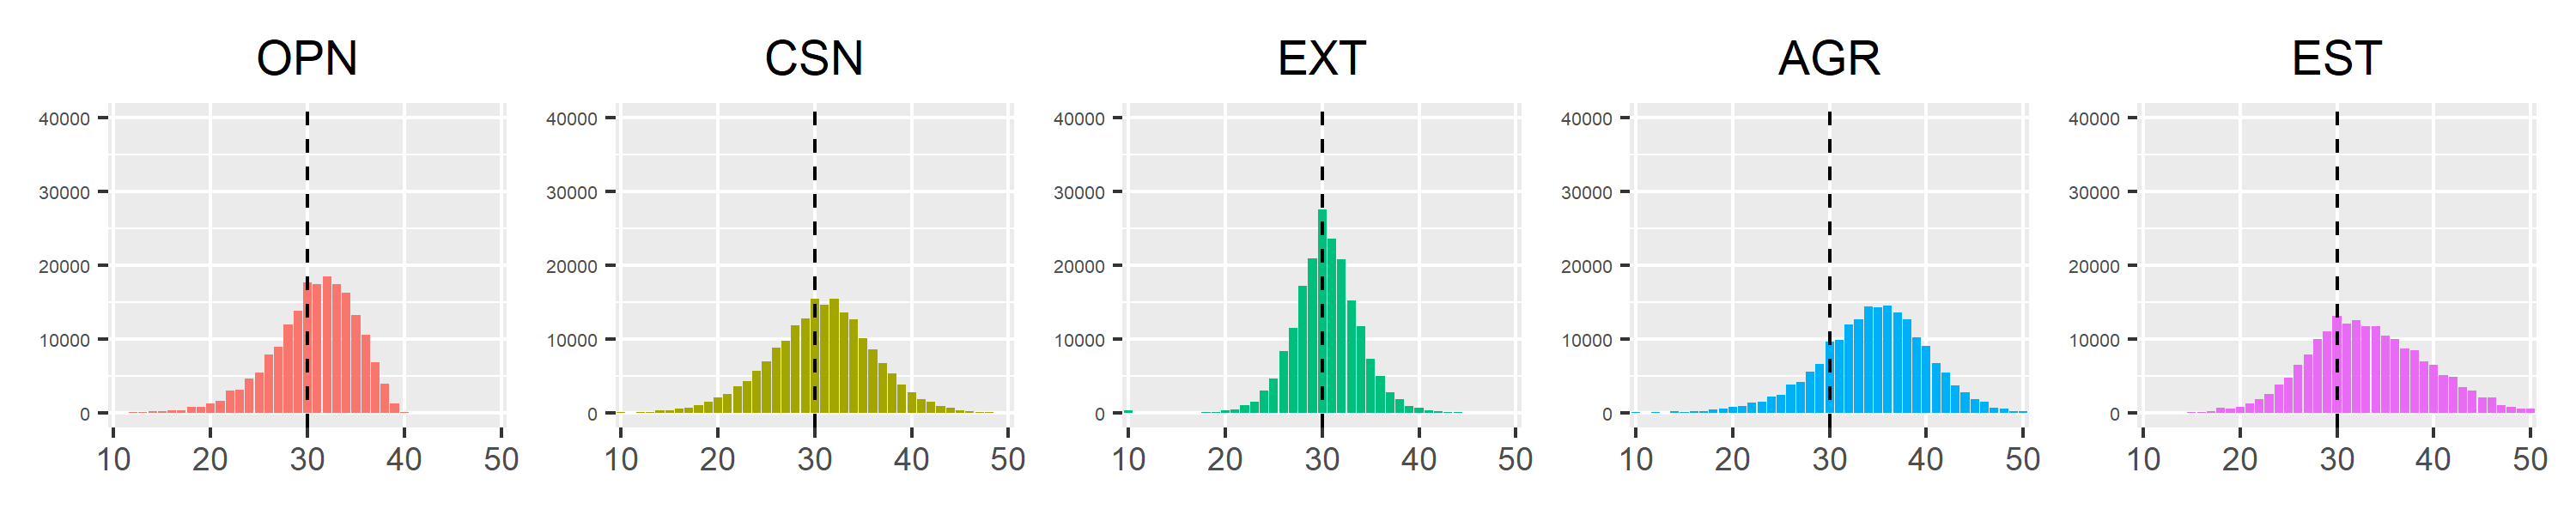
\includegraphics[scale=0.478]{Cluster5.png}
  \caption{类1(189021个样品)的分布}
\end{figure}
如图所示,在不同的类中,分数的最大密度区间有所不同。
以维度总分的中值30为界,将分布图像分成两个部分,定义“绝大部分”为“80\%”。
如果绝大部分样品的维度总分不大于30,记为符号“-”,表示低分倾向;
如果绝大部分样品的维度总分不小于30,记为符号“+”,表示高分倾向;
否则,记为符号“0”,表示中立倾向,可以得到一个关于类的特征的符号矩阵:
\begin{longtable}{c|c|c|c|c|c}
  \hline
  类编号 & OPN & CSN & EXT & AGR & EST \\\hline
  1   & +   & +   & 0   & +   & +   \\
  2   & +   & -   & 0   & +   & +   \\
  3   & +   & +   & 0   & +   & -   \\\hline
  4   & +   & 0   & 0   & 0   & 0   \\
  5   & 0   & 0   & 0   & +   & 0   \\\hline
  \caption{5-均值聚类结果的符号特征}
  \label{symbol5}
\end{longtable}
结合表\ref{center}和表\ref{symbol5},我们能够比较清楚地看出类与类之间的差别和划分依据。
对比类与类之间维度倾向的差异,五个类又可以分为两个大类:
大类1包括类1、类2和类3,主要差异在尽责性维度和宜人性维度,其余维度差别较小;
大类2包括类4和类5,主要差异在开放性维度和宜人性维度,其余维度差别较小。
对比维度在划分类中的重要性,尽责性维度和情绪性维度分出了高分倾向、中立倾向和低分倾向,
区分了两个大类和大类1中的三个小类;
开放性维度和宜人性维度分出了高分倾向和中立倾向,仅区分了大类2中的两个小类。\par
从维度的倾向特征来看,尽责性和外倾性是区分不同人格特质的比较重要的维度,
仅以这两个维度上分数的高低表现就可以将参加测验者大致分入四个类中;
开放性和宜人性是在人格特质中区分度较低的维度,绝大部分人在这两个维度上都有高分倾向;
而外倾性维度在5-均值聚类方法中无法有效区分出不同的人格特质倾向。
\section{十六型人格的聚类}
不同的人格理论可以看作研究人格的不同角度,虽然各个理论描述人格的方法不完全一致,
但既然研究对象同为人类性格,“类型说”和“人格说”的人格测验应该存在某种联系。
目前最热门的人格测验是MBTI十六型人格,那么也许同样可以依据Big5人格测验的结果将人格分成16个类型。\par
对数据进行16-均值聚类,迭代收敛后,16个类分别为:
\begin{longtable}{c|c|c}
  \hline
  类编号 & 样品数   & 类内平方和    \\\hline
  1   & 57111 & 13566.60 \\\hline
  2   & 63403 & 14298.62 \\\hline
  3   & 73622 & 13247.78 \\\hline
  4   & 36915 & 9864.78  \\\hline
  5   & 42954 & 11207.37 \\\hline
  6   & 64605 & 11102.45 \\\hline
  7   & 71200 & 13757.09 \\\hline
  8   & 61827 & 12023.10 \\\hline
  9   & 71959 & 10064.71 \\\hline
  10  & 47915 & 12236.17 \\\hline
  11  & 41432 & 11026.07 \\\hline
  12  & 83898 & 14471.60 \\\hline
  13  & 67361 & 12172.47 \\\hline
  14  & 83729 & 11454.87 \\\hline
  15  & 71569 & 11765.32 \\\hline
  16  & 68690 & 12915.96 \\\hline
  \caption{16-均值聚类结果}
\end{longtable}
\noindent 其中每个类的样品数和类内平方和都在同一水平。类的中心分别为:
\begin{longtable}{c|c|c|c|c|c}
  \hline
  类编号 & OPN   & CSN   & EXT   & AGR   & EST   \\\hline
  1   & 29.34 & 31.02 & 29.88 & 29.65 & 29.23 \\\hline
  2   & 31.34 & 27.86 & 30.57 & 36.29 & 40.91 \\\hline
  3   & 32.27 & 38.31 & 30.81 & 40.15 & 35.45 \\\hline
  4   & 41.99 & 26.02 & 29.78 & 26.39 & 23.46 \\\hline
  5   & 40.61 & 25.05 & 29.01 & 26.94 & 39.99 \\\hline
  6   & 34.52 & 26.22 & 30.98 & 40.01 & 29.33 \\\hline
  7   & 42.93 & 24.27 & 29.83 & 41.56 & 39.93 \\\hline
  8   & 42.55 & 28.91 & 30.78 & 40.60 & 19.81 \\\hline
  9   & 43.26 & 32.21 & 30.80 & 44.83 & 30.07 \\\hline
  10  & 42.08 & 40.17 & 30.18 & 28.21 & 20.69 \\\hline
  11  & 40.82 & 39.53 & 29.27 & 26.57 & 37.30 \\\hline
  12  & 33.76 & 37.97 & 31.03 & 39.79 & 23.25 \\\hline
  13  & 43.00 & 42.37 & 31.20 & 44.20 & 18.03 \\\hline
  14  & 41.51 & 32.96 & 30.50 & 35.17 & 31.73 \\\hline
  15  & 42.12 & 42.98 & 30.70 & 42.94 & 30.07 \\\hline
  16  & 42.47 & 37.13 & 30.12 & 42.14 & 41.60 \\\hline
  % 1   & 40.83 & 39.47 & 29.24 & 26.41 & 37.35 \\\hline
  % 2   & 42.07 & 25.60 & 29.91 & 28.17 & 22.79 \\\hline
  % 3   & 43.21 & 37.76 & 30.06 & 42.26 & 41.10 \\\hline
  % 4   & 41.43 & 25.07 & 29.87 & 41.18 & 41.63 \\\hline
  % 5   & 33.38 & 38.89 & 30.98 & 39.92 & 23.89 \\\hline
  % 6   & 32.61 & 37.70 & 31.04 & 40.14 & 37.04 \\\hline
  % 7   & 41.72 & 25.23 & 29.08 & 27.31 & 38.93 \\\hline
  % 8   & 42.09 & 30.76 & 30.92 & 41.53 & 19.87 \\\hline
  % 9   & 42.27 & 40.11 & 30.15 & 27.90 & 20.70 \\\hline
  % 10  & 33.61 & 27.29 & 31.05 & 40.14 & 29.46 \\\hline
  % 11  & 44.02 & 27.80 & 30.50 & 43.56 & 31.29 \\\hline
  % 12  & 29.77 & 31.52 & 29.88 & 29.44 & 28.33 \\\hline
  % 13  & 42.93 & 42.99 & 31.19 & 44.08 & 17.83 \\\hline
  % 14  & 42.34 & 41.38 & 30.80 & 43.86 & 29.61 \\\hline
  % 15  & 41.05 & 33.89 & 30.59 & 35.48 & 31.41 \\\hline
  % 16  & 30.11 & 27.01 & 30.08 & 34.02 & 40.47 \\\hline
  \caption{16-均值聚类中心}
\end{longtable}
同样以维度总分的中值30为界,将分布图像分成两个部分,
按照生成表\ref{symbol5}的规则,得到关于类的特征的符号矩阵:
\begin{longtable}{c|c|c|c|c|c}
  \hline
  类编号 & OPN & CSN & EXT & AGR & EST \\\hline
  1   & 0   & 0   & 0   & 0   & 0   \\
  2   & 0   & 0   & 0   & +   & +   \\
  3   & 0   & +   & 0   & +   & +   \\
  4   & +   & -   & 0   & 0   & -   \\
  5   & +   & -   & 0   & 0   & +   \\
  6   & +   & -   & 0   & +   & 0   \\
  7   & +   & -   & 0   & +   & +   \\
  8   & +   & 0   & 0   & +   & -   \\
  9   & +   & 0   & 0   & +   & 0   \\
  10  & +   & +   & 0   & 0   & -   \\
  11  & +   & +   & 0   & 0   & +   \\
  12  & +   & +   & 0   & +   & -   \\
  13  & +   & +   & 0   & +   & -   \\
  14  & +   & +   & 0   & +   & 0   \\
  15  & +   & +   & 0   & +   & 0   \\
  16  & +   & +   & 0   & +   & +   \\\hline
  \caption{16-均值聚类结果的符号特征}
  \label{symbol16}
\end{longtable}
从表\ref{symbol16}中可以发现,16个类对于Big5人格测验数据的聚类来说略多,
其中类12和类13、类14和类15没有足够明显的特征差异,
但我们可以从16-均值聚类的结果中得到一些有用的信息。\par
第一,在提高到16个类后,外倾性维度在各个类之间的区分度依旧很低,在各类的分布图像都是对称的钟形。
一种可能的情况是,外倾性是人格中相对独立的一个方面,
一个人对外界的反应是热情或是冷静,并不影响他的开放或保守、尽责或粗心、亲切或严肃、焦躁或镇定。\par
第二,开放性维度和宜人性维度没有分离出具有低分倾向的类。
通过维度和题目的描述我们能看出来,在开放性维度和宜人性维度上有高分倾向的人,
正是社会中比较受欢迎的类型——思想活跃、容易相处,也有很多人想把自己改造为这样的类型;
而老实本分的人多少有些沉闷,斗争性强的人则普遍评价不会太高,社会留给他们的位置相对更少一些。
这种环境下,两个维度出现大量高分倾向的人也就不足为奇了。\par
第三,区分度最好的维度是尽责性维度和情绪性维度。
如果将社会比作一部机器,尽责性维度上的高分人群构成了机器的骨架,低分人群则是润滑剂,
二者都在维系机器正常运行中发挥着作用。
“情绪化”一词更像是一个中性词,它如何发挥作用取决于外部条件。
艺术创作需要丰富的情绪来激发灵感,体育运动需要刺激兴奋来激发潜力,
学习研究需要适当的压力来推动进度,而任何时候面对突发情况又都需要一颗清醒的头脑去处理问题。
因此,社会对在尽责性维度和情绪性维度上具有高分或低分倾向的人有着更高的容忍度,
人们不需要过多地压抑自己的情绪,所以在不同倾向上的分布会更加均匀,容易成为聚类的关键变量。
\part{结论}
% 我们从小到大一直在不断学习知识、与人交往,也许一个人可以考试得到满分、受到周围人的一致好评,
一名专家可以说他很了解自己的研究领域,但很少有人能完整地了解一个人的人格品质,
甚至我们对自己的了解程度也很难说有多高。然而,人与人之间的人格、性格、行为客观上存在着巨大的差异。
当越来越多的人开始对自己、对他人的人格特质感兴趣,
伴随着网络的普及,人格测验逐渐从心理学研究进入到普通人的生活中。\par
得益于测验结果的简洁明了,MBTI十六型人格测验逐渐被大多数人了解和接受,
经常能看到有人展示自己以4个字母代表的人格类型。
这种标签化、脸谱化的人格标签却是与人格的多样化相悖的。
首先,16个类型相对于几十亿人类来说还是太少了,即便被打上同样的类型标签,
两个人可能依旧在某些特质上差异巨大,同时人类社会也一直在不断变化,不断衍生出新的特质组合。
其次,MBTI测验是根据问题的回答得出动力($Energy$)、信息($Information$)、决策($Decision$)、
执行($Execution$)四个维度的倾向,这一点和Big5测验类似,
但之后采用“一刀切”的方式将每个维度一分为二,不管在一个方向上的倾向是1还是99,
都会被记为同一个字母,信息损失非常高,也容易造成结果不准确。
再次,MBTI人格测验结果经常会伴随着一份关于职业、兴趣、交友等方方面面的衍生报告,
这本来是其优势之一,为测试者提供一些建议和参考,并立体化地展示测试者的人格,
可是一旦这份报告被人奉为真理,比如公司根据人格类型招聘、人们一心要从事推荐的职业、
朋友一定要找类型相匹配的,这种僵化的思维势必会造成问题。
最后,由于巴纳姆效应的存在,人们可能轻易就接受了MBTI测验给自己打上的标签,
并且会不断尝试用自己所属的标签来解释自己的行为,认为自己的优点是与生俱来的、缺点是理所当然的,
甚至暗示自己要表现得更符合自己的标签描述,不愿意进一步地改进提升和发掘潜力。\par
本报告主要研究了另一种、被认为更科学的“Big5人格测验”。
Big5人格测验的结果本质上是一个人的行为有何种倾向的可能性,
比如一个人在开放性维度有高分倾向,我们可以说他更可能采取打破常规、有开创性的激进行为,
反之,低分倾向者则更可能采取稳妥的保守行为。
Big5人格测验没有以“贴标签”的形式给人们划分类型,它使用代表“行为可能性”的5个维度分数作为人格指标,
具有实际意义和统计学意义。
除了科学的测验结果,Big5人格测验的评分体系也更加科学,
每个维度包含的题目数量一样,且题目回答采用“五点量表”,
方便了数据化处理,可以直接用题目分数的和作为维度总分,分数即具有相同的量纲。
% 每个维度的题目数量一致——汇总得到的维度总分有相同的量纲,
% 题目的选项一致——容易对选项进行数据化处理,
% 选项与分数1$\sim$5一一对应——可以直接求和计算维度总分。
其次,有了一个人行为倾向的分数,可以进一步联系到他适合什么样的职业和岗位,
Big5人格测验给出了测试者的行为倾向程度,可以提醒人们平时应注意哪方面要谨慎不犯错,
哪方面应尽情发挥,也可以作为如何改变性格的依据。
最后,人格测验的根本目的不是找到最准确的词汇来描述一个人,而是了解他的行为模式,
以期能够在合适的时间作出最合适的行为,而Big5人格测验提供了测试者的行为“可能性”,
或者说,采取各种行为的“概率”,是比较直观的人格描述。\par
时代在不断进步,随着心理学研究的深入,还会有更新、更科学、更准确的人格测验被开发出来。
但就目前来说,Big5人格测验是其中的佼佼者,它理应得到更广泛的认同和应用。
\end{document}